% =============================================================================
%  E1_REP_BDII4_RENFE_MEM  ·  Memoria de la Práctica 1 (repesca)
%  Compilar con pdfLaTeX (Overleaf: Menu > Compiler > pdfLaTeX)
%  Figuras en figuras/: logo_uvigo.png y eer.pdf (diagrama EER vectorial)
% =============================================================================
\documentclass[11pt,a4paper]{article}

% ---------- idioma y tipografía ----------
\usepackage[T1]{fontenc}
\usepackage[utf8]{inputenc}
\usepackage{babel}
\babelprovide[import,main]{spanish}
\IfFileExists{XCharter.sty}{\usepackage{XCharter}}{\usepackage{charter}}
\IfFileExists{beramono.sty}{\usepackage[scaled=0.85]{beramono}}{\usepackage{courier}}
\usepackage{microtype}
\usepackage{newunicodechar}
\newunicodechar{≥}{\ensuremath{\geq}}
\newunicodechar{≤}{\ensuremath{\leq}}
\newunicodechar{≠}{\ensuremath{\neq}}
\newunicodechar{→}{\ensuremath{\rightarrow}}
\newunicodechar{−}{\ensuremath{-}}
\newunicodechar{·}{\ensuremath{\cdot}}
\newunicodechar{€}{\texteuro}

% ---------- página ----------
\usepackage[a4paper,top=2.6cm,bottom=2.6cm,left=2.5cm,right=2.5cm,headheight=14pt]{geometry}
\usepackage{fancyhdr}
\usepackage{titlesec}
\usepackage{xcolor}
\definecolor{azuluvigo}{RGB}{0,51,102}
\definecolor{grisclaro}{RGB}{242,242,242}

% ---------- tablas y figuras ----------
\usepackage{graphicx}
\usepackage{float}
\usepackage{array,tabularx,longtable,booktabs,multirow}
\usepackage{caption}
\captionsetup{font=small,labelfont={bf,color=azuluvigo},justification=raggedright,singlelinecheck=false}
\captionsetup[table]{name=Tabla,position=top}
\captionsetup[figure]{name=Figura}
\usepackage{pdflscape}
\usepackage[section]{placeins}
\usepackage{enumitem}
\setlist{itemsep=2pt,topsep=4pt}
\usepackage{listings}
\lstset{basicstyle=\ttfamily\footnotesize,breaklines=true,frame=single,
        backgroundcolor=\color{grisclaro},rulecolor=\color{gray!50},
        columns=fullflexible,keepspaces=true,
        literate={á}{{\'a}}1 {é}{{\'e}}1 {í}{{\'i}}1 {ó}{{\'o}}1 {ú}{{\'u}}1 {ñ}{{\~n}}1}
\usepackage{tcolorbox}
\usepackage[hidelinks]{hyperref}
\hypersetup{pdftitle={BDII4 RENFE - Practica 1 EER y DDL (repesca)},pdfauthor={Grupo BDII4}}

\renewcommand{\arraystretch}{1.25}
% permitir cortes de línea tras el guion bajo en nombres largos de columnas
\DeclareRobustCommand{\_}{\textunderscore\allowbreak}
\pdfstringdefDisableCommands{\def\_{\textunderscore}}
\setlength{\parskip}{4pt}
\setlength{\parindent}{0pt}
\setlength{\emergencystretch}{2.5em}

\titleformat{\section}{\Large\bfseries\color{azuluvigo}}{\thesection.}{0.6em}{}
\titleformat{\subsection}{\large\bfseries\color{azuluvigo}}{\thesubsection.}{0.6em}{}
\titleformat{\subsubsection}{\normalsize\bfseries}{\thesubsubsection.}{0.6em}{}

\pagestyle{fancy}
\fancyhf{}
\fancyhead[L]{\small\color{gray}BDII4 :: RENFE}
\fancyhead[R]{\small\color{gray}Práctica 1 · EER y DDL · Repesca}
\fancyfoot[C]{\small\thepage}
\renewcommand{\headrulewidth}{0.4pt}

% ---------- utilidades ----------
\newcommand{\RN}[1]{\textbf{RN-#1}}
\newcommand{\tb}[1]{\texttt{#1}}
\newcommand{\figura}[3]{% fichero, ancho, texto si falta
  \IfFileExists{figuras/#1}{\includegraphics[width=#2,height=0.80\textheight,keepaspectratio]{figuras/#1}}%
  {\fbox{\parbox[c][6cm][c]{0.9\linewidth}{\centering\color{red}\bfseries #3}}}}

% ampliación de una zona del EER: trim (izq. abajo der. arriba, en pt), pie, etiqueta
\newcommand{\zoomeer}[3]{%
  \thispagestyle{empty}%
  \centering
  \IfFileExists{figuras/eer.pdf}%
    {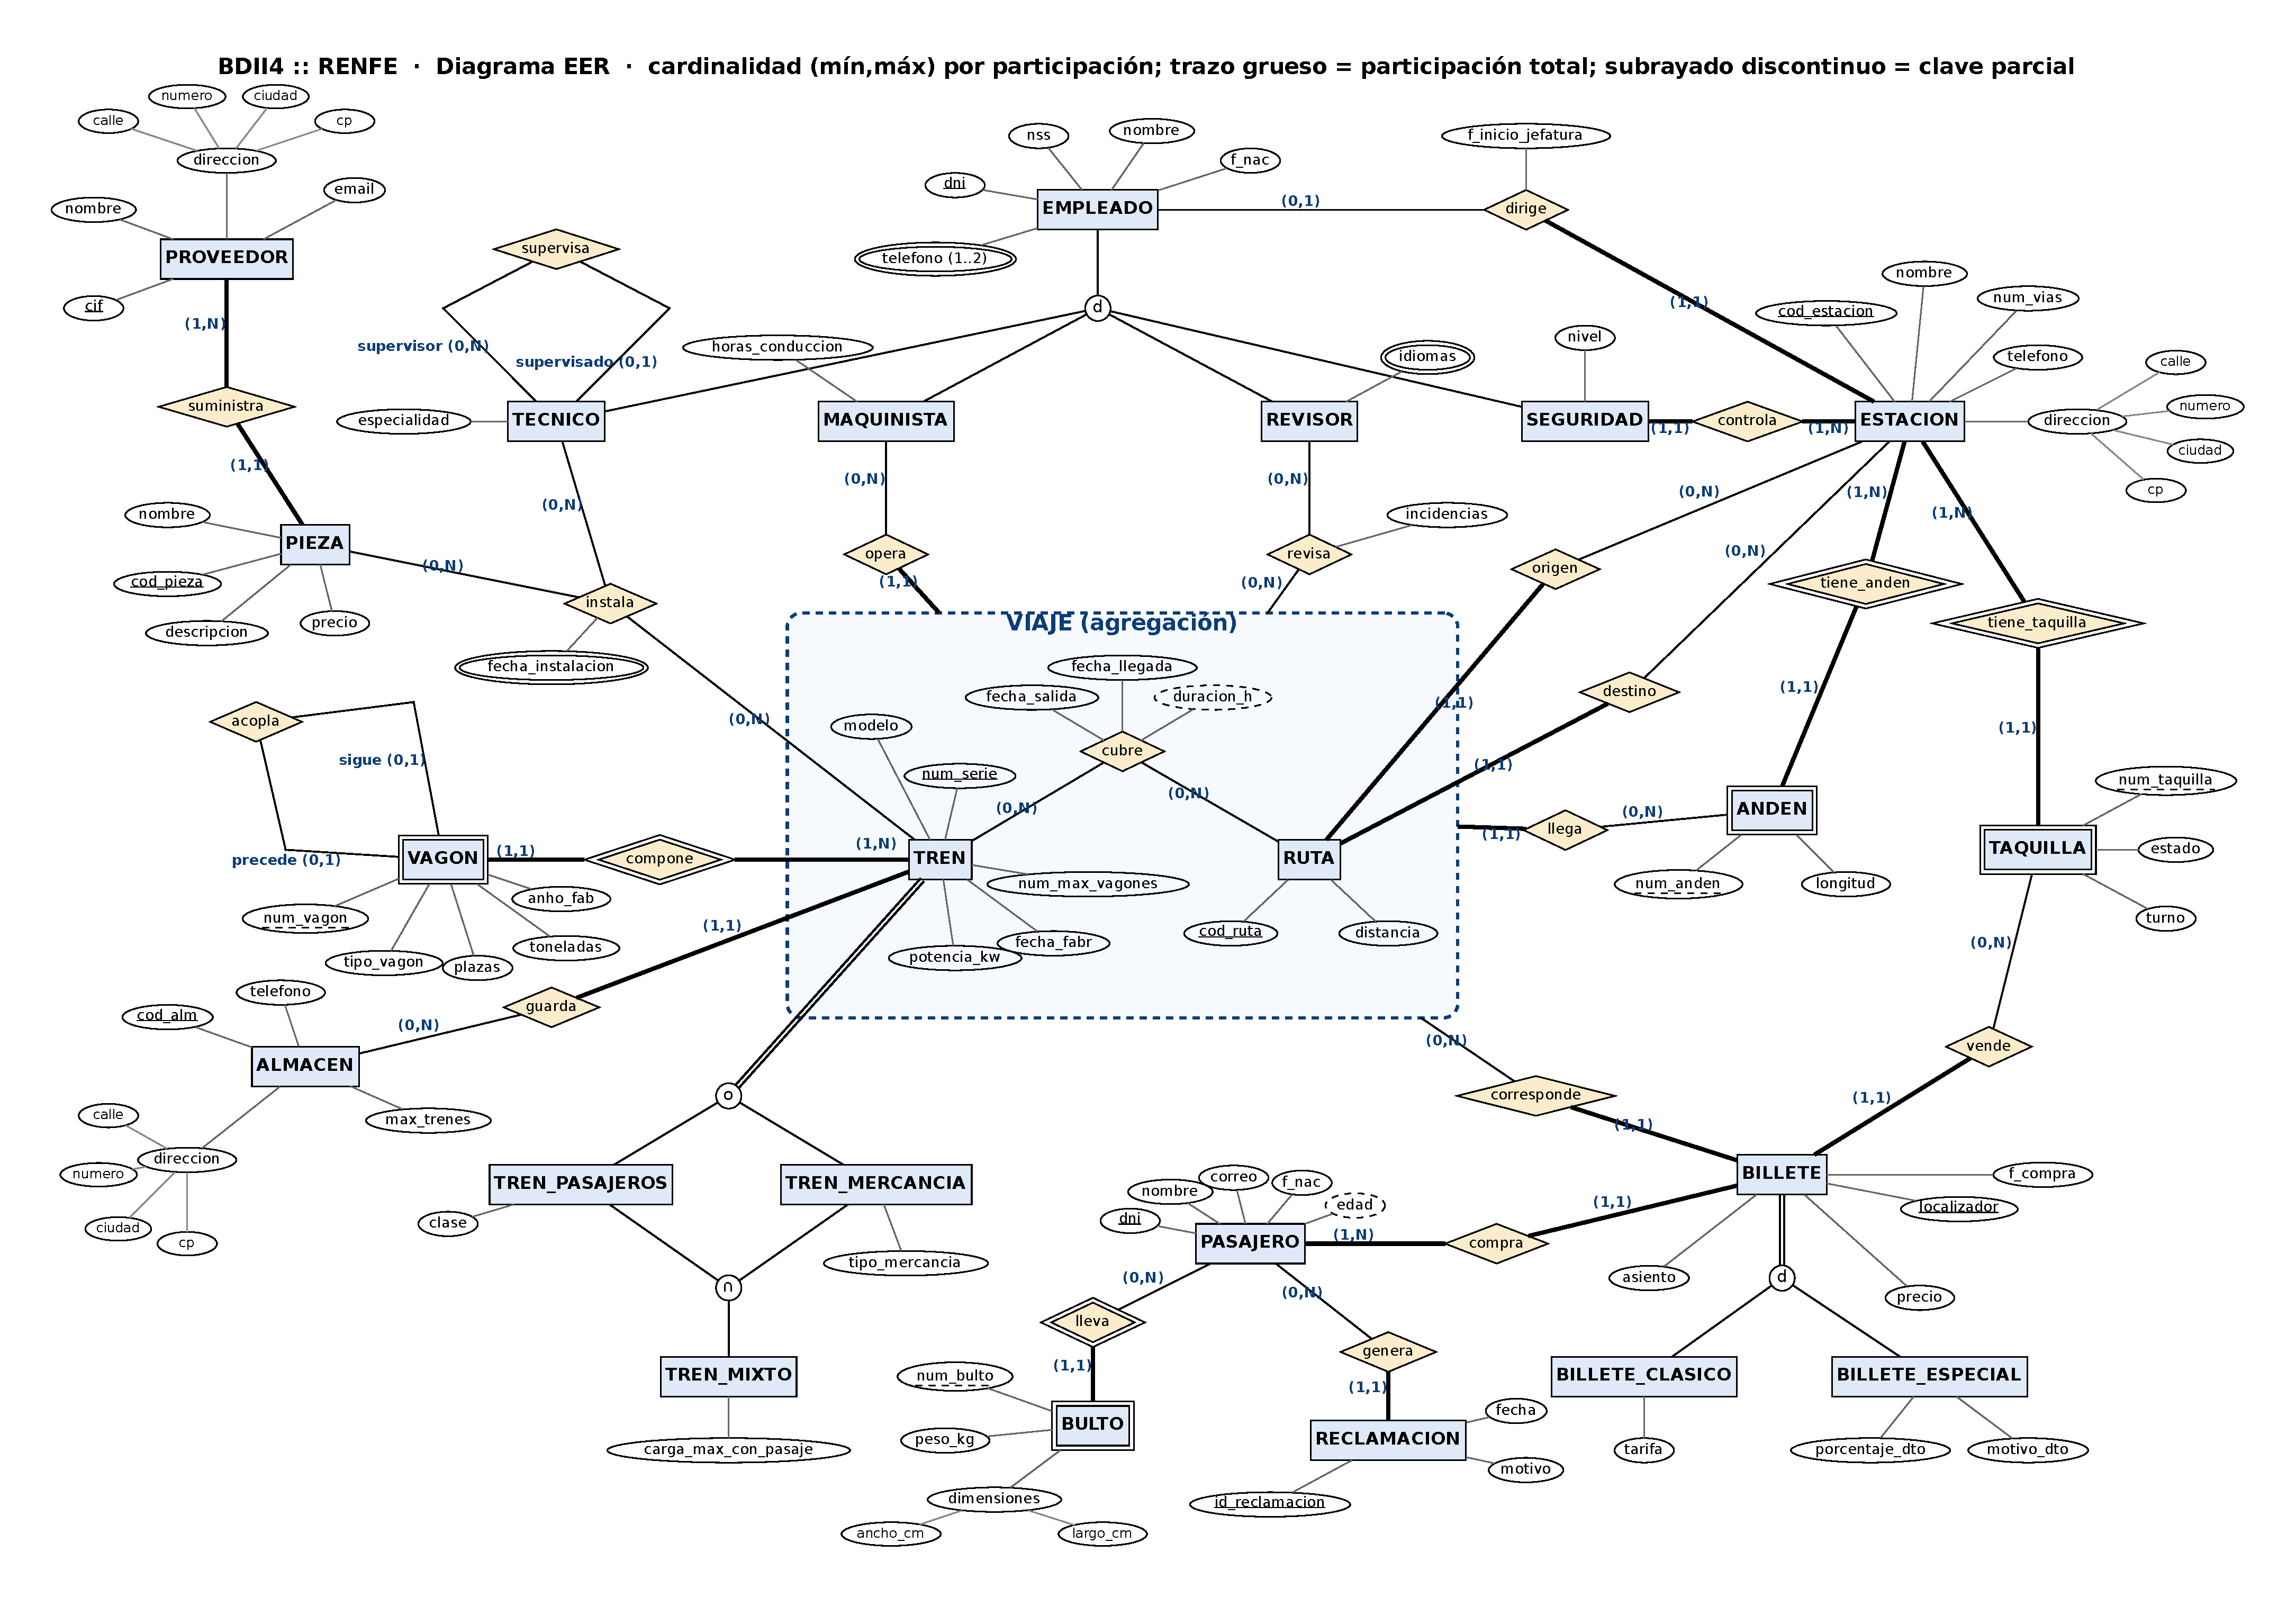
\includegraphics[width=\linewidth,height=0.9\textheight,keepaspectratio,trim=#1,clip]{figuras/eer.pdf}}%
    {\fbox{\parbox[c][8cm][c]{0.8\linewidth}{\centering\color{red}\bfseries Falta figuras/eer.pdf}}}
  \captionof{figure}{#2}\label{#3}}

% =============================================================================
\begin{document}

% ------------------------------ PORTADA --------------------------------------
\begin{titlepage}
\centering
\IfFileExists{figuras/logo_uvigo.png}{
\includegraphics[height=4.2cm]{figuras/logo_uvigo.png}}{}\par
\vspace{0.6cm}
{\Large\scshape Universidade de Vigo}\par
\vspace{0.15cm}
{\large\scshape Escola Superior de Enxeñaría Informática}\par
\vspace{0.15cm}
{\normalsize Bases de Datos II · Curso 2026/2027}\par
\vspace{2.2cm}
{\color{azuluvigo}\rule{\linewidth}{1.2pt}}\par
\vspace{0.4cm}
{\Huge\bfseries Práctica 1: EER y DDL\par}
\vspace{0.3cm}
{\Large Diseño EER, paso al modelo relacional e implantación en Oracle 26ai\par}
\vspace{0.4cm}
{\color{azuluvigo}\rule{\linewidth}{1.2pt}}\par
\vspace{1.2cm}
\begin{tabular}{rl}
\textbf{Código del equipo:} & BDII4 \\
\textbf{Temática:} & RENFE \\
\textbf{Entrega:} & Repesca del Entregable 1 \\
\end{tabular}
\vfill
{\large
Alejandro Francisco Pérez Rodríguez\\[3pt]
Mario Pérez González\\[3pt]
Jacobo Montero Naranjo\\[3pt]
Pablo Regueira Castaño\par}
\vspace{1.2cm}
{\large \today\par}
\end{titlepage}

\tableofcontents
\clearpage

% =============================================================================
\section{Descripción del problema}
% =============================================================================
El sistema da soporte a la operación de una red ferroviaria de viajeros y mercancías. Los actores que intervienen son los \emph{pasajeros}, que compran billetes en las taquillas de las estaciones, viajan con su equipaje y pueden presentar reclamaciones; los \emph{empleados}, organizados por función (maquinistas, revisores, técnicos de mantenimiento y personal de seguridad, además de los jefes de estación); y los \emph{proveedores}, que suministran las piezas de repuesto.

La información que el sistema debe conservar se organiza en cinco áreas: la infraestructura (estaciones, andenes, taquillas y almacenes), el material rodante (trenes y vagones), la explotación (rutas y viajes), la comercialización (pasajeros, billetes, equipaje y reclamaciones) y el mantenimiento (piezas, proveedores e instalaciones realizadas por los técnicos).

\subsection{Reglas de negocio}
Las reglas se numeran en el orden en que se presentan y cada una se referencia en la tabla de justificación (apartado~\ref{sec:justificacion}).

\subsubsection*{Infraestructura}
\begin{description}[leftmargin=1.4cm,style=nextline]
\item[\RN{01}] Una \textbf{estación} se identifica por su código. Se registran su nombre, el número de vías operativas, un teléfono y su dirección, formada por calle, número, ciudad y código postal.
\item[\RN{02}] Un \textbf{andén} se identifica por su número dentro de la estación a la que pertenece y se registra su longitud en metros. Toda estación tiene al menos un andén y cada andén pertenece a una única estación, fuera de la cual no existe.
\item[\RN{03}] Una \textbf{taquilla} se identifica por su número dentro de su estación. Se registran su estado (abierta, cerrada o en mantenimiento) y el turno de operación (mañana, tarde o noche). Toda estación dispone de al menos una taquilla y cada taquilla pertenece a una única estación.
\item[\RN{04}] Un \textbf{almacén} de cocheras se identifica por su código. Se registran su teléfono, la capacidad máxima de trenes y su dirección (calle, número, ciudad y código postal). Un almacén puede estar vacío o guardar varios trenes.
\end{description}

\subsubsection*{Personal}
\begin{description}[leftmargin=1.4cm,style=nextline]
\item[\RN{05}] Un \textbf{empleado} se identifica por su DNI; su número de la Seguridad Social también es único. Se registran su nombre, su fecha de nacimiento y entre uno y dos teléfonos de contacto. Según su función, un empleado puede ser \textbf{maquinista} (horas de conducción), \textbf{revisor} (idiomas que domina, uno o varios), \textbf{técnico} (especialidad) o de \textbf{seguridad} (nivel asignado, de 1 a 5). Un empleado desempeña como máximo uno de estos roles y puede no desempeñar ninguno, como ocurre con los jefes de estación.
\item[\RN{06}] Cada estación está \textbf{dirigida} por exactamente un empleado (jefe de estación) y un empleado dirige como máximo una estación. Se registra la fecha en que comenzó la jefatura. La jefatura es un cargo de gestión: el jefe de estación no desempeña ninguno de los cuatro roles operativos de \RN{05}.
\item[\RN{07}] Cada empleado de \textbf{seguridad} controla una única estación, y toda estación cuenta con al menos un empleado de seguridad.
\item[\RN{08}] Los técnicos se organizan jerárquicamente: un técnico puede \textbf{supervisar} a varios técnicos y cada técnico tiene como máximo un supervisor. Los técnicos de mayor rango no tienen supervisor y ningún técnico se supervisa a sí mismo.
\end{description}

\subsubsection*{Material rodante}
\begin{description}[leftmargin=1.4cm,style=nextline]
\item[\RN{09}] Un \textbf{tren} se identifica por su número de serie. Se registran su modelo, su potencia en kW, su fecha de fabricación y el número máximo de vagones. Cada tren se guarda en un único almacén.
\item[\RN{10}] Todo tren es de \textbf{pasajeros} (se registra su clase de servicio), de \textbf{mercancías} (se registra el tipo de mercancía) o de ambos tipos a la vez.
\item[\RN{11}] Los trenes que son a la vez de pasajeros y de mercancías son \textbf{trenes mixtos}. Para ellos se registra la carga máxima, en toneladas, autorizada cuando circulan con viajeros a bordo. Este dato no tiene sentido para ningún otro tren.
\item[\RN{12}] Un \textbf{vagón} se identifica por su número dentro del tren al que pertenece. Se registran su tipo (pasajeros, restaurante o mercancías), su capacidad (en plazas para los de pasajeros y restaurante, en toneladas para los de mercancías) y su año de fabricación. Todo tren tiene al menos un vagón y cada vagón pertenece a un único tren.
\item[\RN{13}] Dentro de un tren, cada vagón tiene como máximo un vagón \textbf{acoplado} a continuación (si no lo tiene, es el último) y como máximo uno delante (si no lo tiene, es el primero). Ambos vagones pertenecen siempre al mismo tren.
\end{description}

\subsubsection*{Explotación}
\begin{description}[leftmargin=1.4cm,style=nextline]
\item[\RN{14}] Una \textbf{ruta} se identifica por su código y se registra su distancia en kilómetros. Toda ruta parte de una única estación de \textbf{origen} y termina en una única estación de \textbf{destino}, que son distintas. Una estación puede no ser origen ni destino de ninguna ruta o serlo de varias.
\item[\RN{15}] Un tren \textbf{cubre} una ruta en una fecha y hora de salida concretas, con su fecha y hora de llegada; la duración en horas se obtiene de ambas. Un tren puede no haber cubierto ninguna ruta (tren nuevo o en taller) o cubrir muchas, y una ruta puede no haberse operado todavía o ser cubierta por varios trenes. Cada cobertura concreta es un \textbf{viaje}, que se relaciona como un objeto con el personal, los billetes y los andenes.
\item[\RN{16}] Cada viaje es \textbf{conducido} por exactamente un maquinista. Un maquinista puede conducir ningún viaje (recién incorporado) o muchos.
\item[\RN{17}] Un viaje puede ser \textbf{revisado} por varios revisores o por ninguno, porque los trenes de mercancías no llevan revisor. Un revisor puede revisar ningún viaje o muchos. Por cada revisor y viaje se registra el número de incidencias detectadas.
\item[\RN{18}] Cada viaje \textbf{llega} a un único andén, que pertenece a la estación de destino de su ruta. Un andén puede recibir ningún viaje o muchos.
\end{description}

\subsubsection*{Comercialización}
\begin{description}[leftmargin=1.4cm,style=nextline]
\item[\RN{19}] Un \textbf{pasajero} se identifica por su DNI; su correo electrónico es único. Se registran su nombre y su fecha de nacimiento, de la que se obtiene su edad.
\item[\RN{20}] Un \textbf{billete} se identifica por su localizador. Se registran la fecha de compra, el precio abonado y el asiento. Cada billete lo \textbf{vende} una única taquilla, lo \textbf{compra} un único pasajero y \textbf{corresponde} a un único viaje. Una taquilla puede no haber vendido ningún billete; un pasajero se registra al comprar su primer billete, por lo que tiene al menos uno; un viaje puede no tener billetes (los de mercancías no los tienen). Un mismo asiento no puede venderse dos veces para el mismo viaje.
\item[\RN{21}] Todo billete es \textbf{clásico} (se registra su tarifa: Básico, Elige o Prémium) o \textbf{especial} (se registran el porcentaje de descuento y su motivo), nunca ambos.
\item[\RN{22}] Un \textbf{bulto} se identifica por su número dentro del pasajero que lo porta. Se registran su peso en kg y sus dimensiones (ancho y largo en cm). Un pasajero puede viajar sin bultos o con varios.
\item[\RN{23}] Una \textbf{reclamación} se identifica por su código. Se registran la fecha en que se presenta y el motivo. Cada reclamación la \textbf{genera} un único pasajero; un pasajero puede no generar ninguna o generar varias.
\end{description}

\subsubsection*{Mantenimiento}
\begin{description}[leftmargin=1.4cm,style=nextline]
\item[\RN{24}] Un \textbf{proveedor} se identifica por su CIF. Se registran su nombre comercial, su correo de contacto y su dirección (calle, número, ciudad y código postal). Un proveedor \textbf{suministra} al menos una pieza y cada pieza la suministra un único proveedor.
\item[\RN{25}] Una \textbf{pieza} se identifica por su código. Se registran su nombre comercial, una descripción técnica y su precio unitario.
\item[\RN{26}] Un técnico \textbf{instala} una pieza en un tren. Un técnico puede no haber realizado instalaciones (recién incorporado) o muchas; una pieza puede no haberse instalado nunca o instalarse en varias ocasiones; un tren puede no haber recibido piezas o recibir varias. Se registran las fechas de instalación, que pertenecen a la combinación de técnico, pieza y tren y no a ninguno de ellos por separado. Una misma combinación puede repetirse en fechas distintas (por ejemplo, las pastillas de freno se sustituyen periódicamente), así que cada combinación tiene una o varias fechas.
\end{description}

\subsection{Supuestos}
\begin{itemize}
\item Los viajes, billetes, instalaciones y reclamaciones son registros históricos: no se eliminan al dar de baja las entidades relacionadas.
\item El jefe de estación es un cargo de gestión independiente de los cuatro roles operativos, por lo que los jefes son empleados sin rol operativo (\RN{05}, \RN{06}). Puede haber además otros empleados de gestión sin rol.
\item Una pieza representa un tipo de repuesto del catálogo, no una unidad física; por eso puede instalarse varias veces, incluso en el mismo tren y por el mismo técnico (\RN{26}).
\item Las estaciones de origen y destino de una ruta son estaciones de la red registradas en el sistema (\RN{14}).
\item La convención de cardinalidad es la de \emph{participación} (mínimo, máximo): el par junto a una entidad indica en cuántas instancias de la relación participa cada ocurrencia de esa entidad. Todas las cardinalidades son contiguas.
\end{itemize}

\clearpage
% =============================================================================
\section{Diagrama Entidad-Relación Extendido}
% =============================================================================
\subsection{Diagrama}
La Figura~\ref{fig:eer} muestra el modelo completo como vista global. Como a tamaño A4 el texto de la vista global es pequeño, las Figuras~\ref{fig:eer-z1} a~\ref{fig:eer-z4} amplían el mismo diagrama por zonas, de modo que todo se lee al 100\,\%. Las ampliaciones se solapan ligeramente para que cada relación aparezca completa en al menos una de ellas. El diagrama es un gráfico vectorial y puede ampliarse además sin pérdida de calidad.

Notación empleada: rectángulo doble para las entidades débiles y rombo doble para su relación identificadora; elipse doble para los atributos multivaluados y discontinua para los derivados; identificadores con subrayado continuo y claves parciales de las entidades débiles con subrayado discontinuo; trazo grueso para la participación total; círculo \emph{d} u \emph{o} para las especializaciones disjuntas o solapadas, con doble línea hacia la superclase cuando son totales; círculo $\cap$ para la subclase compartida; y caja discontinua para la agregación Viaje. Cada par (mín,máx) indica la participación de la entidad junto a la que aparece.



\subsection{Recuento de mínimos}
\begin{table}[H]
\centering\small
\caption{Comprobación de los requisitos mínimos del enunciado.}
\label{tab:minimos}
\begin{tabularx}{\linewidth}{>{\raggedright\arraybackslash}p{4.4cm} c >{\raggedright\arraybackslash}X}
\toprule
\textbf{Requisito} & \textbf{Mín.} & \textbf{En el modelo} \\
\midrule
Tipos de entidad & 12 & 23: 14 entidades (Estación, Andén, Taquilla, Almacén, Tren, Vagón, Ruta, Empleado, Pasajero, Bulto, Billete, Reclamación, Pieza, Proveedor) y 9 subclases (Maquinista, Revisor, Técnico, Seguridad, Tren\_Pasajeros, Tren\_Mercancía, Tren\_Mixto, Billete\_Clásico, Billete\_Especial) \\
Entidades débiles & 2 & 4: Andén, Taquilla, Vagón y Bulto, con clave parcial, relación identificadora y participación total \\
Especializaciones / generalizaciones & 2 & 3: Empleado (disjunta, parcial), Tren (solapada, total) y Billete (disjunta, total) \\
Constructos extendidos de tipos distintos & 2 & Agregación Viaje y subclase compartida Tren\_Mixto \\
Relaciones & 10 & 21 \\
Relaciones 1:1 & 2 & 2: DIRIGE y ACOPLA \\
Relaciones 1:N & 2 & 16: TIENE\_ANDEN, TIENE\_TAQUILLA, COMPONE, LLEVA, SUPERVISA, CONTROLA, GUARDA, ORIGEN, DESTINO, OPERA, LLEGA, VENDE, COMPRA, CORRESPONDE, GENERA, SUMINISTRA \\
Relaciones N:M & 2 & 2: CUBRE y REVISA \\
Relaciones reflexivas & 2 & 2: ACOPLA (Vagón, roles precede/sigue) y SUPERVISA (Técnico, roles supervisor/supervisado) \\
Relación ternaria & 1 & INSTALA (Técnico, Pieza, Tren) \\
Relaciones con atributos propios & 2 & 4: CUBRE (fechas de salida y llegada, duración), REVISA (incidencias), INSTALA (fechas de instalación), DIRIGE (fecha de inicio de jefatura) \\
Atributo compuesto & 1 & dirección (Estación, Almacén, Proveedor) y dimensiones (Bulto) \\
Atributo multivaluado & 1 & teléfono (Empleado, 1 a 2 valores), idiomas (Revisor) y fecha\_instalacion (INSTALA) \\
Atributo derivado & 1 & duración (CUBRE/Viaje) y edad (Pasajero) \\
Participación total y parcial en especializaciones & 1 + 1 & Total: Tren y Billete; parcial: Empleado \\
Cardinalidad (mín,máx) en todas las participaciones & -- & Sí, con la convención de participación (contigua) indicada en los supuestos \\
\bottomrule
\end{tabularx}
\end{table}

Ningún elemento se ha añadido solo para alcanzar un mínimo: todos proceden de una regla de negocio.

\paragraph{Elementos que cubren más de un mínimo.} El enunciado solo lo admite cuando es semánticamente correcto y se justifica, así que se indica expresamente:
\begin{itemize}
\item \textbf{ACOPLA} es a la vez reflexiva y 1:1. Relaciona vagones con vagones (reflexiva) y cada vagón tiene como máximo uno delante y uno detrás (\RN{13}), luego ambos máximos son 1. Es la segunda 1:1 junto con DIRIGE, así que el mínimo de dos 1:1 se apoya en ella. Es correcto porque las dos propiedades se deducen directamente de \RN{13} y ninguna cardinalidad se ha forzado para el recuento.
\item \textbf{SUPERVISA} es a la vez reflexiva y 1:N, porque un técnico supervisa a varios y tiene como máximo un supervisor (\RN{08}). Las 1:N no dependen de ella: hay otras quince.
\item \textbf{CUBRE} es la N:M agregada en Viaje y tiene atributos propios. Que sea N:M y tenga atributos se deduce de \RN{15}; la agregación es necesaria porque otras relaciones se asocian con cada cobertura concreta. El mínimo de relaciones con atributos no depende de ella (hay otras tres).
\item \textbf{INSTALA} es la ternaria y además tiene atributos propios. El mínimo de relaciones con atributos tampoco depende de ella.
\end{itemize}

\newgeometry{margin=0.8cm}
\begin{landscape}
\thispagestyle{empty}
\centering
\IfFileExists{figuras/eer.pdf}%
  {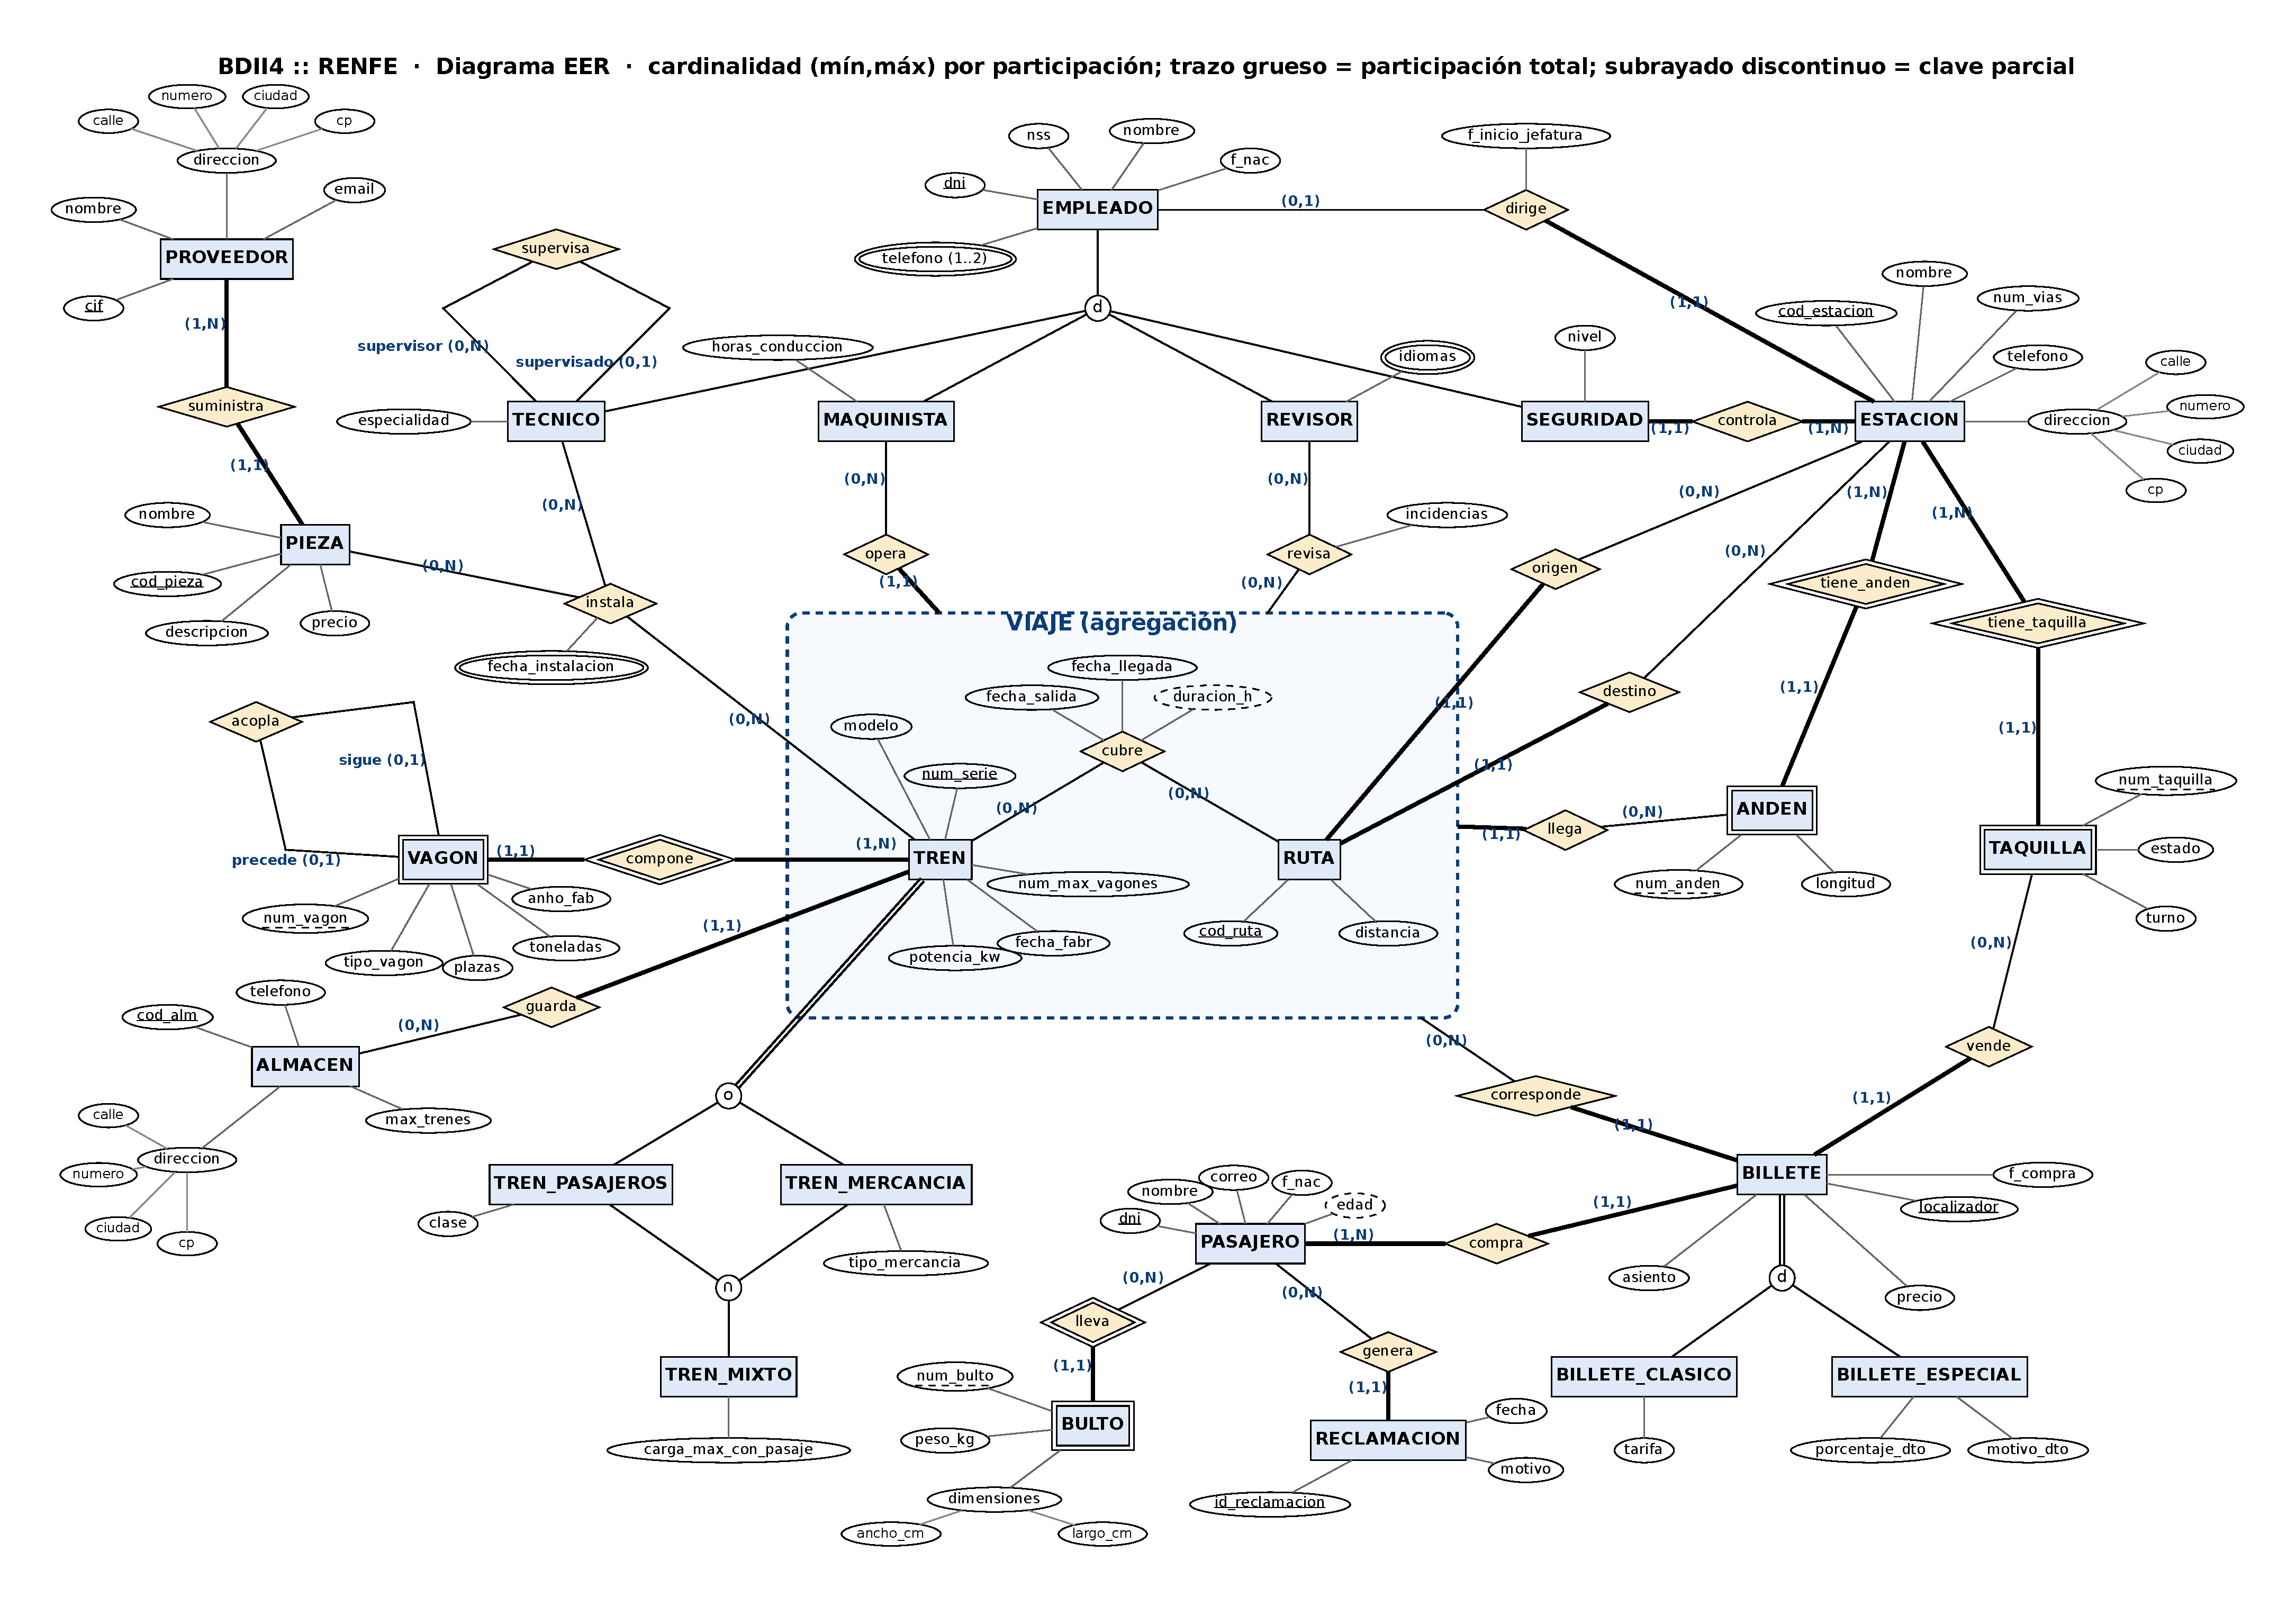
\includegraphics[width=\linewidth,height=0.93\textheight,keepaspectratio]{figuras/eer.pdf}}%
  {\fbox{\parbox[c][8cm][c]{0.8\linewidth}{\centering\color{red}\bfseries Falta figuras/eer.pdf}}}
\captionof{figure}{Diagrama EER completo (vista global). Las Figuras~\ref{fig:eer-z1} a~\ref{fig:eer-z4} lo amplían por zonas.}
\label{fig:eer}
\newpage
\zoomeer{0 681 958 0}{Ampliación 1 de 4 del EER: personal (especialización de Empleado, SUPERVISA, OPERA) y mantenimiento (Proveedor, Pieza, ternaria INSTALA).}{fig:eer-z1}
\newpage
\zoomeer{958 637 0 0}{Ampliación 2 de 4 del EER: estaciones y rutas (DIRIGE, CONTROLA, REVISA, Andén y Taquilla, ORIGEN y DESTINO, LLEGA).}{fig:eer-z2}
\newpage
\zoomeer{0 0 958 594}{Ampliación 3 de 4 del EER: material rodante (Vagón y ACOPLA, Almacén, generalización de Tren y subclase compartida Tren\_Mixto) y agregación Viaje.}{fig:eer-z3}
\newpage
\zoomeer{958 0 0 710}{Ampliación 4 de 4 del EER: comercialización (Pasajero, Bulto, Reclamación, Billete y su especialización, VENDE, COMPRA, CORRESPONDE).}{fig:eer-z4}
\end{landscape}
\restoregeometry



\subsection{Tabla de justificación}
\label{sec:justificacion}
{\small
\begin{longtable}{>{\raggedright\arraybackslash}p{2.9cm} >{\raggedright\arraybackslash}p{1.1cm} >{\raggedright\arraybackslash}p{3.3cm} >{\raggedright\arraybackslash}p{6.6cm}}
\caption{Justificación de las decisiones del EER.}\label{tab:justif}\\
\toprule
\textbf{Elemento} & \textbf{Regla} & \textbf{Decisión} & \textbf{Justificación} \\
\midrule
\endfirsthead
\toprule
\textbf{Elemento} & \textbf{Regla} & \textbf{Decisión} & \textbf{Justificación} \\
\midrule
\endhead
\bottomrule
\endfoot
Especialización de Empleado & RN-05, RN-06 & Disjunta (d) y parcial & \emph{Criterio de pertenencia}: la función operativa que desempeña el empleado (definida por el usuario al asignarle el rol). Disjunta porque cada empleado desempeña como máximo un rol operativo. Parcial porque existen empleados sin rol operativo, como los jefes de estación (RN-06). Cada subclase tiene atributos o relaciones propios. \\
Generalización de Tren & RN-10 & Solapada (o) y total & \emph{Criterio de pertenencia}: el tipo de servicio que presta el tren (viajeros, mercancías o ambos), definido por el usuario. Total porque no existen trenes que no sean de pasajeros ni de mercancías. Solapada porque un tren puede ser de ambos tipos a la vez. \\
Especialización de Billete & RN-21 & Disjunta (d) y total & \emph{Criterio de pertenencia}: la modalidad comercial con la que se vende el billete (clásica o especial), definida por el usuario en la venta. Total porque todo billete se vende en una de las dos modalidades; disjunta porque se excluyen. Cada subclase tiene atributos propios (tarifa; porcentaje y motivo). \\
Subclase compartida Tren\_Mixto & RN-11 & Subclase de Tren\_Pasajeros y de Tren\_Mercancía & Sus miembros pertenecen a la intersección de ambas subclases y heredan los atributos de las dos. Necesita representarse aparte porque tiene un atributo propio (carga máxima con pasaje) que no tiene sentido en ningún otro tren. \\
Agregación Viaje & RN-15 a RN-18, RN-20 & CUBRE tratada como entidad de nivel superior & El maquinista, los revisores, el andén de llegada y los billetes se asocian a un viaje concreto (tren + ruta + salida), no al tren ni a la ruta por separado. Sin agregación habría que usar relaciones de grado 4 o superior con información redundante. \\
Andén (débil) & RN-02 & Clave parcial num\_anden; TIENE\_ANDEN identificadora; Andén (1,1), Estación (1,N) & Su número solo es único dentro de la estación y no existe fuera de ella. \\
Taquilla (débil) & RN-03 & Clave parcial num\_taquilla; TIENE\_TAQUILLA; Taquilla (1,1), Estación (1,N) & Igual que el andén: se numera por estación y depende de ella. \\
Vagón (débil) & RN-12 & Clave parcial num\_vagon; COMPONE; Vagón (1,1), Tren (1,N) & Los vagones se numeran por tren y no se registran sin el tren al que pertenecen. \\
Bulto (débil) & RN-22 & Clave parcial num\_bulto; LLEVA; Bulto (1,1), Pasajero (0,N) & El bulto se numera por pasajero y solo interesa mientras está asociado a él. \\
Ternaria INSTALA & RN-26 & Técnico (0,N), Pieza (0,N), Tren (0,N); atributo multivaluado fecha\_instalacion & Con tres binarias (Técnico–Pieza, Pieza–Tren, Técnico–Tren) se sabría qué piezas toca un técnico y qué piezas recibe un tren, pero no qué técnico instaló qué pieza en qué tren ni en qué fecha: las binarias no permiten reconstruir la terna. Ejemplo: si A instala P1 en T1 y P2 en T2, y B instala P1 en T2, las binarias también contienen (A, P1, T2), que nunca ocurrió. Las fechas dependen de la combinación de las tres entidades; son multivaluadas porque la misma terna se repite en el tiempo (RN-26). \\
Reflexiva ACOPLA & RN-13 & 1:1; precede (0,1), sigue (0,1) & Cada vagón tiene como máximo uno detrás y uno delante; el 0 corresponde al primer y al último vagón. Los dos roles distinguen la posición relativa. \\
Reflexiva SUPERVISA & RN-08 & 1:N; supervisor (0,N), supervisado (0,1) & Un técnico supervisa a varios y tiene como máximo un supervisor. El mínimo 0 del supervisado es necesario: si fuera 1, la cadena de supervisión no tendría fin. \\
DIRIGE & RN-06 & 1:1; Empleado (0,1), Estación (1,1); atributo f\_inicio\_jefatura & Toda estación tiene un jefe y un empleado dirige como máximo una estación; la mayoría de empleados no dirige ninguna. La fecha depende de la pareja empleado–estación. Participa la superclase Empleado porque el jefe no tiene rol operativo. \\
CONTROLA & RN-07 & 1:N; Seguridad (1,1), Estación (1,N) & Todo vigilante está asignado a una estación y toda estación tiene al menos uno. \\
GUARDA & RN-04, RN-09 & 1:N; Almacén (0,N), Tren (1,1) & Un almacén puede estar vacío; todo tren tiene un almacén asignado. \\
ORIGEN y DESTINO & RN-14 & Dos 1:N; Estación (0,N), Ruta (1,1) en cada una & Los extremos de una ruta son estaciones de la red, así que se modelan como relaciones con Estación y no como texto: cada concepto se representa una sola vez. Son dos relaciones distintas porque tienen significado distinto; una estación puede no ser extremo de ninguna ruta. \\
CUBRE & RN-15 & N:M; Tren (0,N), Ruta (0,N); fechas y duración & Ni el tren ni la ruta están obligados a participar (tren en taller, ruta nueva). Las fechas pertenecen a cada cobertura; la duración es derivada. \\
OPERA & RN-16 & 1:N; Maquinista (0,N), Viaje (1,1) & Todo viaje tiene un único maquinista; un maquinista puede no tener viajes asignados. \\
REVISA & RN-17 & N:M; Revisor (0,N), Viaje (0,N); atributo incidencias & Varios revisores pueden controlar un mismo viaje y un revisor controla muchos. Viaje participa con mínimo 0 porque los trenes de mercancías no llevan revisor. Las incidencias dependen de la pareja revisor–viaje. \\
LLEGA & RN-18 & 1:N; Viaje (1,1), Andén (0,N) & La llegada es del viaje concreto, no del tren: el mismo tren llega a andenes distintos en viajes distintos. Que el andén sea de la estación destino de la ruta no se ve en el diagrama (apartado~\ref{sec:noexpresa}). \\
VENDE & RN-20 & 1:N; Taquilla (0,N), Billete (1,1) & Una taquilla nueva o cerrada puede no haber vendido billetes. \\
COMPRA & RN-20 & 1:N; Pasajero (1,N), Billete (1,1) & El pasajero se registra al comprar; todo billete tiene un único comprador. \\
CORRESPONDE & RN-20 & 1:N; Viaje (0,N), Billete (1,1) & Cada billete es para un viaje; los viajes de mercancías no tienen billetes. Que un pasajero realiza un viaje se deduce de sus billetes, sin relación adicional. \\
GENERA & RN-23 & 1:N; Pasajero (0,N), Reclamación (1,1) & Las reclamaciones son opcionales para el pasajero y siempre tienen autor. \\
SUMINISTRA & RN-24 & 1:N; Proveedor (1,N), Pieza (1,1) & Un proveedor solo se registra si suministra; cada pieza tiene un proveedor exclusivo. \\
\midrule
Atributo compuesto dirección; dimensiones & RN-01, RN-04, RN-24; RN-22 & Compuestos & La dirección se usa completa (envíos, localización) pero también por partes (búsquedas por ciudad o código postal). Las dimensiones del bulto se comprueban por separado (ancho y largo). \\
Atributos multivaluados teléfono, idiomas y fecha\_instalacion & RN-05; RN-26 & Multivaluados & Un empleado tiene uno o dos teléfonos y un revisor domina uno o varios idiomas; una misma instalación (terna) se repite en varias fechas. Un atributo simple obligaría a fijar un número de columnas o a perder valores. \\
Atributos derivados duracion\_h y edad & RN-15; RN-19 & Derivados & Se calculan a partir de las fechas de salida y llegada y de la fecha de nacimiento. Almacenarlos duplicaría información y la edad quedaría desactualizada. \\
\end{longtable}
}

\subsection{Restricciones que el EER no expresa gráficamente}
\label{sec:noexpresa}
\begin{itemize}
\item En ACOPLA, los dos vagones deben pertenecer al mismo tren y no puede formarse un ciclo (\RN{13}).
\item El número de vagones de un tren no puede superar \tb{num\_max\_vagones} (\RN{09}) ni el número de trenes de un almacén su \tb{max\_trenes} (\RN{04}).
\item La capacidad de un vagón se mide en plazas o en toneladas según su tipo (\RN{12}).
\item Un asiento no se vende dos veces en el mismo viaje (\RN{20}).
\item El andén de llegada de un viaje pertenece a la estación de destino de su ruta (\RN{18}).
\item La fecha de llegada de un viaje es posterior a la de salida, y las estaciones de origen y destino de una ruta son distintas (\RN{14}, \RN{15}).
\item Los jefes de estación no tienen rol operativo (\RN{06}).
\item Un tren que es a la vez de pasajeros y de mercancías figura como tren mixto (\RN{11}): la subclase compartida indica qué trenes \emph{pueden} ser mixtos, no que todos los de la intersección lo sean.
\end{itemize}

% =============================================================================
\section{Transformación al modelo relacional}
% =============================================================================
\subsection{Esquema relacional}
Notación: clave primaria \underline{subrayada}, claves foráneas en \textit{cursiva}. Bajo cada relación se indican sus claves foráneas, con la acción de borrado aplicada, y sus claves candidatas.

{\small\begin{longtable}{@{}>{\raggedright\arraybackslash}p{\linewidth}@{}}
\textbf{EMPLEADO}(\underline{dni}, nss, nombre, f\_nac, tipo\_empleado)\newline{\footnotesize\quad Clave candidata: (nss)} \\[4pt]
\textbf{EMPLEADO\_TELEFONO}(\underline{\textit{dni\_empleado}}, \underline{orden}, telefono)\newline{\footnotesize\quad FK (dni\_empleado) $\rightarrow$ EMPLEADO [ON DELETE CASCADE]\newline\quad Clave candidata: (dni\_empleado, telefono)} \\[4pt]
\textbf{ESTACION}(\underline{cod\_estacion}, nombre, calle, numero, ciudad, cp, num\_vias, telefono, \textit{dni\_jefe}, f\_inicio\_jefatura)\newline{\footnotesize\quad FK (dni\_jefe) $\rightarrow$ EMPLEADO [sin acción]\newline\quad Clave candidata: (dni\_jefe)} \\[4pt]
\textbf{MAQUINISTA}(\underline{\textit{dni}}, \textit{tipo\_empleado}, horas\_conduccion)\newline{\footnotesize\quad FK (dni, tipo\_empleado) $\rightarrow$ EMPLEADO [ON DELETE CASCADE]} \\[4pt]
\textbf{REVISOR}(\underline{\textit{dni}}, \textit{tipo\_empleado})\newline{\footnotesize\quad FK (dni, tipo\_empleado) $\rightarrow$ EMPLEADO [ON DELETE CASCADE]} \\[4pt]
\textbf{REVISOR\_IDIOMA}(\underline{\textit{dni\_revisor}}, \underline{idioma})\newline{\footnotesize\quad FK (dni\_revisor) $\rightarrow$ REVISOR [ON DELETE CASCADE]} \\[4pt]
\textbf{TECNICO}(\underline{\textit{dni}}, \textit{tipo\_empleado}, especialidad, \textit{dni\_supervisor})\newline{\footnotesize\quad FK (dni, tipo\_empleado) $\rightarrow$ EMPLEADO [ON DELETE CASCADE]\newline\quad FK (dni\_supervisor) $\rightarrow$ TECNICO [ON DELETE SET NULL]} \\[4pt]
\textbf{SEGURIDAD}(\underline{\textit{dni}}, \textit{tipo\_empleado}, nivel, \textit{cod\_estacion})\newline{\footnotesize\quad FK (dni, tipo\_empleado) $\rightarrow$ EMPLEADO [ON DELETE CASCADE]\newline\quad FK (cod\_estacion) $\rightarrow$ ESTACION [sin acción]} \\[4pt]
\textbf{ANDEN}(\underline{\textit{cod\_estacion}}, \underline{num\_anden}, longitud)\newline{\footnotesize\quad FK (cod\_estacion) $\rightarrow$ ESTACION [ON DELETE CASCADE]} \\[4pt]
\textbf{TAQUILLA}(\underline{\textit{cod\_estacion}}, \underline{num\_taquilla}, estado, turno)\newline{\footnotesize\quad FK (cod\_estacion) $\rightarrow$ ESTACION [ON DELETE CASCADE]} \\[4pt]
\textbf{ALMACEN}(\underline{cod\_alm}, telefono, max\_trenes, calle, numero, ciudad, cp) \\[4pt]
\textbf{PASAJERO}(\underline{dni}, nombre, correo, f\_nac)\newline{\footnotesize\quad Clave candidata: (correo)} \\[4pt]
\textbf{RUTA}(\underline{cod\_ruta}, \textit{cod\_estacion\_origen}, \textit{cod\_estacion\_destino}, distancia)\newline{\footnotesize\quad FK (cod\_estacion\_origen) $\rightarrow$ ESTACION [sin acción]\newline\quad FK (cod\_estacion\_destino) $\rightarrow$ ESTACION [sin acción]\newline\quad UNIQUE (cod\_ruta, cod\_estacion\_destino), superclave referenciada por VIAJE} \\[4pt]
\textbf{PROVEEDOR}(\underline{cif}, nombre, email, calle, numero, ciudad, cp) \\[4pt]
\textbf{PIEZA}(\underline{cod\_pieza}, nombre, descripcion, precio, \textit{cif\_proveedor})\newline{\footnotesize\quad FK (cif\_proveedor) $\rightarrow$ PROVEEDOR [sin acción]} \\[4pt]
\textbf{BULTO}(\underline{\textit{dni\_pasajero}}, \underline{num\_bulto}, peso\_kg, ancho\_cm, largo\_cm)\newline{\footnotesize\quad FK (dni\_pasajero) $\rightarrow$ PASAJERO [ON DELETE CASCADE]} \\[4pt]
\textbf{RECLAMACION}(\underline{id\_reclamacion}, fecha, motivo, \textit{dni\_pasajero})\newline{\footnotesize\quad FK (dni\_pasajero) $\rightarrow$ PASAJERO [sin acción]} \\[4pt]
\textbf{TREN}(\underline{num\_serie}, modelo, potencia\_kw, fecha\_fabr, num\_max\_vagones, \textit{cod\_alm})\newline{\footnotesize\quad FK (cod\_alm) $\rightarrow$ ALMACEN [sin acción]} \\[4pt]
\textbf{TREN\_PASAJEROS}(\underline{\textit{num\_serie}}, clase)\newline{\footnotesize\quad FK (num\_serie) $\rightarrow$ TREN [ON DELETE CASCADE]} \\[4pt]
\textbf{TREN\_MERCANCIA}(\underline{\textit{num\_serie}}, tipo\_mercancia)\newline{\footnotesize\quad FK (num\_serie) $\rightarrow$ TREN [ON DELETE CASCADE]} \\[4pt]
\textbf{TREN\_MIXTO}(\underline{\textit{num\_serie}}, carga\_max\_con\_pasaje)\newline{\footnotesize\quad FK (num\_serie) $\rightarrow$ TREN\_PASAJEROS [ON DELETE CASCADE]\newline\quad FK (num\_serie) $\rightarrow$ TREN\_MERCANCIA [ON DELETE CASCADE]} \\[4pt]
\textbf{VAGON}(\underline{\textit{num\_serie\_tren}}, \underline{num\_vagon}, tipo\_vagon, plazas, toneladas, anho\_fab, \textit{vagon\_sig\_num})\newline{\footnotesize\quad FK (num\_serie\_tren) $\rightarrow$ TREN [ON DELETE CASCADE]\newline\quad FK (num\_serie\_tren, vagon\_sig\_num) $\rightarrow$ VAGON [sin acción]} \\[4pt]
\textbf{INSTALACION}(\underline{\textit{dni\_tecnico}}, \underline{\textit{cod\_pieza}}, \underline{\textit{num\_serie\_tren}}, \underline{fecha\_instalacion})\newline{\footnotesize\quad Ternaria INSTALA con su multivaluado fecha\_instalacion (ver decisiones de transformación)\newline\quad FK (dni\_tecnico) $\rightarrow$ TECNICO [sin acción]\newline\quad FK (cod\_pieza) $\rightarrow$ PIEZA [sin acción]\newline\quad FK (num\_serie\_tren) $\rightarrow$ TREN [sin acción]} \\[4pt]
\textbf{VIAJE}(\underline{\textit{num\_serie\_tren}}, \underline{\textit{cod\_ruta}}, \underline{fecha\_salida}, fecha\_llegada, duracion\_h\textsuperscript{(derivado, columna virtual)}, \textit{dni\_maquinista}, \textit{cod\_estacion\_llegada}, \textit{num\_anden\_llegada})\newline{\footnotesize\quad FK (num\_serie\_tren) $\rightarrow$ TREN [sin acción]\newline\quad FK (cod\_ruta) $\rightarrow$ RUTA [sin acción]\newline\quad FK (dni\_maquinista) $\rightarrow$ MAQUINISTA [sin acción]\newline\quad FK (cod\_estacion\_llegada, num\_anden\_llegada) $\rightarrow$ ANDEN [sin acción]\newline\quad FK (cod\_ruta, cod\_estacion\_llegada) $\rightarrow$ RUTA (cod\_ruta, cod\_estacion\_destino) [sin acción]} \\[4pt]
\textbf{REVISOR\_VIAJE}(\underline{\textit{dni\_revisor}}, \underline{\textit{num\_serie\_tren}}, \underline{\textit{cod\_ruta}}, \underline{\textit{fecha\_salida}}, incidencias)\newline{\footnotesize\quad FK (dni\_revisor) $\rightarrow$ REVISOR [sin acción]\newline\quad FK (num\_serie\_tren, cod\_ruta, fecha\_salida) $\rightarrow$ VIAJE [ON DELETE CASCADE]} \\[4pt]
\textbf{BILLETE}(\underline{localizador}, tipo\_billete, f\_compra, precio, asiento, \textit{cod\_estacion\_taq}, \textit{num\_taquilla}, \textit{dni\_pasajero}, \textit{num\_serie\_tren}, \textit{cod\_ruta}, \textit{fecha\_salida})\newline{\footnotesize\quad FK (cod\_estacion\_taq, num\_taquilla) $\rightarrow$ TAQUILLA [sin acción]\newline\quad FK (dni\_pasajero) $\rightarrow$ PASAJERO [sin acción]\newline\quad FK (num\_serie\_tren, cod\_ruta, fecha\_salida) $\rightarrow$ VIAJE [sin acción]\newline\quad Clave candidata: (num\_serie\_tren, cod\_ruta, fecha\_salida, asiento)} \\[4pt]
\textbf{BILLETE\_CLASICO}(\underline{\textit{localizador}}, \textit{tipo\_billete}, tarifa)\newline{\footnotesize\quad FK (localizador, tipo\_billete) $\rightarrow$ BILLETE [ON DELETE CASCADE]} \\[4pt]
\textbf{BILLETE\_ESPECIAL}(\underline{\textit{localizador}}, \textit{tipo\_billete}, porcentaje\_dto, motivo\_dto)\newline{\footnotesize\quad FK (localizador, tipo\_billete) $\rightarrow$ BILLETE [ON DELETE CASCADE]} \\[4pt]
\end{longtable}}

\subsection{Decisiones de transformación}
\subsubsection*{Entidades y atributos}
\begin{itemize}
\item \textbf{Entidades fuertes}: una relación por entidad, con su identificador como clave primaria. Las claves candidatas (NSS de Empleado, correo de Pasajero) se declaran UNIQUE.
\item \textbf{Atributos compuestos} (dirección, dimensiones): se almacenan sus componentes simples (\tb{calle}, \tb{numero}, \tb{ciudad}, \tb{cp}; \tb{ancho\_cm}, \tb{largo\_cm}).
\item \textbf{Atributos multivaluados}: generan una relación propia cuya clave es la del propietario más el valor (\tb{REVISOR\_IDIOMA}). En \tb{EMPLEADO\_TELEFONO} se usa la clave (dni, orden) con \tb{orden IN (1,2)}, lo que limita de forma declarativa el número de teléfonos a dos, como exige \RN{05}; el par (dni, teléfono) queda como clave candidata. El multivaluado fecha\_instalacion de INSTALA se trata junto con la ternaria.
\item \textbf{Atributos derivados}: la duración del viaje se implanta como columna virtual (\tb{duracion\_h}) que Oracle calcula al consultarla. La edad no puede ser columna virtual porque depende de \tb{SYSDATE}; se calcula en la vista \tb{VISTA\_PASAJERO\_EDAD} a partir de \tb{f\_nac}.
\end{itemize}

\subsubsection*{Entidades débiles}
Andén, Taquilla, Vagón y Bulto generan relaciones cuya clave primaria es la clave del propietario más la clave parcial. La clave del propietario es a la vez clave foránea con \tb{ON DELETE CASCADE}, que refleja la dependencia de existencia.

\subsubsection*{Relaciones binarias}
\begin{itemize}
\item \textbf{1:N}: clave foránea en el lado N. Cuando la participación de ese lado es total (1,1) la columna es \tb{NOT NULL}: Seguridad, Pieza, Reclamación, Tren, Ruta (origen y destino), Viaje (maquinista y andén) y Billete (taquilla, pasajero y viaje).
\item \textbf{ORIGEN y DESTINO}: dos claves foráneas a Estación en Ruta (\tb{cod\_estacion\_origen} y \tb{cod\_estacion\_destino}), cada una con su nombre de rol, y un CHECK que exige que sean distintas.
\item \textbf{1:1 DIRIGE}: la clave foránea se coloca en Estación, el lado con participación total, como \tb{NOT NULL} y \tb{UNIQUE} (el UNIQUE garantiza el máximo 1 del lado Empleado). El atributo de la relación, \tb{f\_inicio\_jefatura}, se coloca junto a ella. Ponerla en Empleado obligaría a admitir nulos en casi todas las filas.
\item \textbf{N:M REVISA}: relación propia \tb{REVISOR\_VIAJE}, con clave formada por la del revisor y la del viaje e incluyendo el atributo \tb{incidencias}.
\end{itemize}

\subsubsection*{Relaciones reflexivas}
\begin{itemize}
\item \textbf{ACOPLA (1:1)}: clave foránea compuesta (\tb{num\_serie\_tren}, \tb{vagon\_sig\_num}) hacia la propia tabla Vagón, lo que obliga a que el vagón siguiente sea del mismo tren. El UNIQUE sobre esas dos columnas garantiza el máximo 1 del rol \emph{sigue}. Como Oracle indexa las claves compuestas parcialmente nulas, el mismo UNIQUE impide además que un tren tenga dos últimos vagones.
\item \textbf{SUPERVISA (1:N)}: columna \tb{dni\_supervisor} en Técnico, admite nulos (supervisado 0,1), con un CHECK que impide la autosupervisión.
\end{itemize}

\subsubsection*{Relación ternaria}
Aplicando el algoritmo, la ternaria INSTALA daría una relación con las claves de las tres entidades y su atributo multivaluado otra cuya clave es la de INSTALA más el valor:
\begin{itemize}
\item \tb{INSTALA}(\underline{dni\_tecnico}, \underline{cod\_pieza}, \underline{num\_serie\_tren})
\item \tb{INSTALACION}(\underline{dni\_tecnico}, \underline{cod\_pieza}, \underline{num\_serie\_tren}, \underline{fecha\_instalacion})
\end{itemize}
Como INSTALA no tiene más atributos y toda terna tiene al menos una fecha, la primera sería exactamente la proyección de la segunda sobre las tres claves: no aporta información y solo duplicaría datos. Por eso se implanta únicamente \tb{INSTALACION}, cuya clave primaria incluye la fecha. Es la transformación del diagrama, no una corrección: la fecha está en la clave porque en el EER es multivaluada.

\subsubsection*{Especializaciones}
\begin{itemize}
\item \textbf{Empleado (disjunta, parcial)}: una relación para la superclase y otra por subclase (opción a). La disyunción se garantiza con un atributo discriminante \tb{tipo\_empleado}, un UNIQUE (dni, tipo\_empleado) en Empleado y una clave foránea compuesta en cada subclase con el tipo fijado por CHECK: un empleado solo puede aparecer en la subclase que indica su tipo. La parcialidad se refleja en que el discriminante admite NULL. Se descarta la tabla única (opciones c y d) porque Seguridad participa en CONTROLA, Maquinista en OPERA y Técnico en SUPERVISA e INSTALA: sus claves foráneas deben apuntar a cada subclase.
\item \textbf{Tren (solapada, total)}: opción a. Es la única que admite el solapamiento sin duplicar los atributos heredados (la opción b los repetiría en dos tablas para los trenes mixtos) ni llenar la tabla de nulos (opción e). La totalidad no se puede expresar declarativamente y se comprueba con una consulta (apartado~\ref{sec:pruebas}).
\item \textbf{Billete (disjunta, total)}: opción a con el mismo discriminante que Empleado, ahora \tb{NOT NULL} para reflejar la totalidad. Se prefiere a la tabla única porque así los atributos propios de cada subclase pueden ser \tb{NOT NULL} en su tabla.
\end{itemize}

\subsubsection*{Constructos extendidos}
\begin{itemize}
\item \textbf{Agregación Viaje}: la N:M CUBRE se transforma en la relación \tb{VIAJE}, con clave (tren, ruta, fecha de salida). Esa clave es la que referencian las relaciones que salen de la agregación: OPERA y LLEGA como claves foráneas dentro de Viaje (Viaje participa con 1,1), CORRESPONDE como clave foránea en Billete y REVISA en \tb{REVISOR\_VIAJE}. La fecha de salida forma parte de la clave porque un tren cubre la misma ruta muchas veces. Para \RN{18} se añade una segunda clave foránea (\tb{cod\_ruta}, \tb{cod\_estacion\_llegada}) hacia (\tb{cod\_ruta}, \tb{cod\_estacion\_destino}) de Ruta, que se declara UNIQUE: así el andén de llegada solo puede estar en la estación destino de la ruta del viaje, de forma declarativa.
\item \textbf{Subclase compartida Tren\_Mixto}: relación con la clave del tren y dos claves foráneas, una a \tb{TREN\_PASAJEROS} y otra a \tb{TREN\_MERCANCIA}. Así solo puede ser tren mixto uno que ya pertenezca a ambas subclases, es decir, a su intersección.
\end{itemize}

\subsection{Restricciones preservadas y comprobación adicional}
\begin{table}[!htbp]
\centering\small
\caption{Restricciones del EER y forma en que se garantizan.}
\begin{tabularx}{\linewidth}{>{\raggedright\arraybackslash}X >{\raggedright\arraybackslash}p{6.4cm}}
\toprule
\textbf{Restricción} & \textbf{Garantía} \\
\midrule
Identificadores, claves parciales y claves candidatas & PK y UNIQUE (declarativa) \\
Participación total del lado N en relaciones 1:N y 1:1 & FK \tb{NOT NULL} (declarativa) \\
Máximo 1 en DIRIGE y ACOPLA & UNIQUE (declarativa) \\
Disyunción de Empleado y de Billete & Discriminante + FK compuesta (declarativa) \\
Pertenencia de Tren\_Mixto a la intersección & Doble FK (declarativa) \\
Máximo de dos teléfonos & PK (dni, orden) + CHECK (declarativa) \\
Dominios, fechas ordenadas, origen distinto del destino, vagón no acoplado a sí mismo, coherencia tipo–capacidad, asiento único por viaje & CHECK y UNIQUE (declarativa) \\
Andén de llegada en la estación destino de la ruta & FK compuesta Viaje $\rightarrow$ Ruta (declarativa) \\
\midrule
Totalidad de Tren y Billete; trenes de ambos tipos registrados como mixtos; jefes sin rol operativo; empleados con al menos un teléfono & Consulta de comprobación (apartado~\ref{sec:pruebas}) \\
Mínimos 1 del lado 1 (estación con andén, taquilla y seguridad; tren con vagón; proveedor con pieza; pasajero con billete; revisor con idioma) & No declarativa: requeriría disparadores; se respeta en los datos de prueba \\
Ausencia de ciclos en ACOPLA y SUPERVISA; \tb{num\_max\_vagones}; \tb{max\_trenes} & No declarativa: requeriría disparadores (ver Limitaciones) \\
\bottomrule
\end{tabularx}
\end{table}

% =============================================================================
\section{Diccionario de datos}
% =============================================================================
Para cada tabla se indican el significado, el tipo Oracle, la nulabilidad y las restricciones de cada atributo. Las restricciones se nombran con los prefijos \tb{pk\_}, \tb{fk\_}, \tb{uq\_}, \tb{nn\_} y \tb{chk\_} seguidos de la tabla y el campo; en las tablas se abrevian cuando el nombre se deduce de la convención.

\begin{table}[!htbp]
\centering\small
\caption{EMPLEADO. Superclase de la especialización parcial y disjunta de empleados (RN-05).}
\label{dic:empleado}
\begin{tabularx}{\linewidth}{>{\raggedright\arraybackslash}p{2.8cm} >{\raggedright\arraybackslash}p{2.75cm} c >{\raggedright\arraybackslash}X >{\raggedright\arraybackslash}X}
\toprule
\textbf{Atributo} & \textbf{Tipo} & \textbf{Nulo} & \textbf{Significado} & \textbf{Restricciones} \\
\midrule
\texttt{dni} & VARCHAR2(9) & No & DNI del empleado & PK pk\_empleado; CHECK formato 8 dígitos + letra (chk\_empleado\_dni) \\
\texttt{nss} & VARCHAR2(12) & No & Número de la Seguridad Social & NN nn\_empleado\_nss; UNIQUE uq\_empleado\_nss; CHECK 12 dígitos (chk\_empleado\_nss) \\
\texttt{nombre} & VARCHAR2(100) & No & Nombre completo & NN nn\_empleado\_nombre \\
\texttt{f\_nac} & DATE & Sí & Fecha de nacimiento & -- \\
\texttt{tipo\_empleado} & VARCHAR2(10) & Sí & Discriminante del rol operativo; NULL si no tiene rol (parcialidad) & CHECK IN (MAQUINISTA, REVISOR, TECNICO, SEGURIDAD) (chk\_empleado\_tipo); UNIQUE (dni, tipo\_empleado) (uq\_empleado\_dni\_tipo) \\
\bottomrule
\end{tabularx}
\end{table}

\begin{table}[!htbp]
\centering\small
\caption{EMPLEADO\_TELEFONO. Atributo multivaluado teléfono de EMPLEADO, entre 1 y 2 valores (RN-05).}
\label{dic:empleado_telefono}
\begin{tabularx}{\linewidth}{>{\raggedright\arraybackslash}p{2.8cm} >{\raggedright\arraybackslash}p{2.75cm} c >{\raggedright\arraybackslash}X >{\raggedright\arraybackslash}X}
\toprule
\textbf{Atributo} & \textbf{Tipo} & \textbf{Nulo} & \textbf{Significado} & \textbf{Restricciones} \\
\midrule
\texttt{dni\_empleado} & VARCHAR2(9) & No & Empleado titular & PK; FK → EMPLEADO ON DELETE CASCADE (fk\_emptel\_empleado) \\
\texttt{orden} & NUMBER(1) & No & Posición del teléfono (1 o 2) & PK; CHECK IN (1,2) (chk\_emptel\_orden): limita a dos teléfonos \\
\texttt{telefono} & VARCHAR2(15) & No & Número de contacto & NN; UNIQUE (dni\_empleado, telefono); CHECK formato numérico 9–14 cifras \\
\bottomrule
\end{tabularx}
\end{table}

\begin{table}[!htbp]
\centering\small
\caption{ESTACION. Entidad fuerte con dirección compuesta; incorpora la relación 1:1 DIRIGE (RN-01, RN-06).}
\label{dic:estacion}
\begin{tabularx}{\linewidth}{>{\raggedright\arraybackslash}p{2.8cm} >{\raggedright\arraybackslash}p{2.75cm} c >{\raggedright\arraybackslash}X >{\raggedright\arraybackslash}X}
\toprule
\textbf{Atributo} & \textbf{Tipo} & \textbf{Nulo} & \textbf{Significado} & \textbf{Restricciones} \\
\midrule
\texttt{cod\_estacion} & VARCHAR2(10) & No & Código de la estación & PK pk\_estacion \\
\texttt{nombre} & VARCHAR2(100) & No & Nombre comercial & NN nn\_estacion\_nombre \\
\texttt{calle, numero, ciudad} & VARCHAR2 (100, 10, 50) & Sí & Componentes de la dirección & -- \\
\texttt{cp} & VARCHAR2(5) & Sí & Código postal (dirección) & CHECK 5 dígitos (chk\_estacion\_cp) \\
\texttt{num\_vias} & NUMBER(3) & Sí & Vías operativas & CHECK > 0 (chk\_estacion\_vias) \\
\texttt{telefono} & VARCHAR2(15) & Sí & Teléfono de contacto & -- \\
\texttt{dni\_jefe} & VARCHAR2(9) & No & Empleado que dirige la estación (DIRIGE) & NN; UNIQUE (uq\_estacion\_jefe); FK → EMPLEADO, sin acción (fk\_estacion\_jefe) \\
\texttt{f\_inicio\_jefatura} & DATE & No & Atributo de DIRIGE: inicio de la jefatura & NN nn\_estacion\_finicio \\
\bottomrule
\end{tabularx}
\end{table}

\begin{table}[!htbp]
\centering\small
\caption{MAQUINISTA. Subclase de EMPLEADO (RN-05).}
\label{dic:maquinista}
\begin{tabularx}{\linewidth}{>{\raggedright\arraybackslash}p{2.8cm} >{\raggedright\arraybackslash}p{2.75cm} c >{\raggedright\arraybackslash}X >{\raggedright\arraybackslash}X}
\toprule
\textbf{Atributo} & \textbf{Tipo} & \textbf{Nulo} & \textbf{Significado} & \textbf{Restricciones} \\
\midrule
\texttt{dni} & VARCHAR2(9) & No & Empleado maquinista & PK; FK (dni, tipo\_empleado) → EMPLEADO ON DELETE CASCADE \\
\texttt{tipo\_empleado} & VARCHAR2(10) & No & Discriminante fijo & DEFAULT y CHECK = MAQUINISTA; NN \\
\texttt{horas\_conduccion} & NUMBER(6) & Sí & Horas de conducción acumuladas & DEFAULT 0; CHECK ≥ 0 \\
\bottomrule
\end{tabularx}
\end{table}

\begin{table}[!htbp]
\centering\small
\caption{REVISOR. Subclase de EMPLEADO (RN-05).}
\label{dic:revisor}
\begin{tabularx}{\linewidth}{>{\raggedright\arraybackslash}p{2.8cm} >{\raggedright\arraybackslash}p{2.75cm} c >{\raggedright\arraybackslash}X >{\raggedright\arraybackslash}X}
\toprule
\textbf{Atributo} & \textbf{Tipo} & \textbf{Nulo} & \textbf{Significado} & \textbf{Restricciones} \\
\midrule
\texttt{dni} & VARCHAR2(9) & No & Empleado revisor & PK; FK (dni, tipo\_empleado) → EMPLEADO ON DELETE CASCADE \\
\texttt{tipo\_empleado} & VARCHAR2(10) & No & Discriminante fijo & DEFAULT y CHECK = REVISOR; NN \\
\bottomrule
\end{tabularx}
\end{table}

\begin{table}[!htbp]
\centering\small
\caption{REVISOR\_IDIOMA. Atributo multivaluado idiomas de REVISOR (RN-05).}
\label{dic:revisor_idioma}
\begin{tabularx}{\linewidth}{>{\raggedright\arraybackslash}p{2.8cm} >{\raggedright\arraybackslash}p{2.75cm} c >{\raggedright\arraybackslash}X >{\raggedright\arraybackslash}X}
\toprule
\textbf{Atributo} & \textbf{Tipo} & \textbf{Nulo} & \textbf{Significado} & \textbf{Restricciones} \\
\midrule
\texttt{dni\_revisor} & VARCHAR2(9) & No & Revisor & PK; FK → REVISOR ON DELETE CASCADE \\
\texttt{idioma} & VARCHAR2(30) & No & Idioma que domina & PK \\
\bottomrule
\end{tabularx}
\end{table}

\begin{table}[!htbp]
\centering\small
\caption{TECNICO. Subclase de EMPLEADO; incluye la reflexiva SUPERVISA (RN-05, RN-08).}
\label{dic:tecnico}
\begin{tabularx}{\linewidth}{>{\raggedright\arraybackslash}p{2.8cm} >{\raggedright\arraybackslash}p{2.75cm} c >{\raggedright\arraybackslash}X >{\raggedright\arraybackslash}X}
\toprule
\textbf{Atributo} & \textbf{Tipo} & \textbf{Nulo} & \textbf{Significado} & \textbf{Restricciones} \\
\midrule
\texttt{dni} & VARCHAR2(9) & No & Empleado técnico & PK; FK (dni, tipo\_empleado) → EMPLEADO ON DELETE CASCADE \\
\texttt{tipo\_empleado} & VARCHAR2(10) & No & Discriminante fijo & DEFAULT y CHECK = TECNICO; NN \\
\texttt{especialidad} & VARCHAR2(100) & Sí & Especialidad técnica & -- \\
\texttt{dni\_supervisor} & VARCHAR2(9) & Sí & Rol supervisor de SUPERVISA; NULL si no tiene & FK reflexiva → TECNICO ON DELETE SET NULL; CHECK ≠ dni (chk\_tecnico\_no\_autosup) \\
\bottomrule
\end{tabularx}
\end{table}

\begin{table}[!htbp]
\centering\small
\caption{SEGURIDAD. Subclase de EMPLEADO; incluye la relación 1:N CONTROLA (RN-05, RN-07).}
\label{dic:seguridad}
\begin{tabularx}{\linewidth}{>{\raggedright\arraybackslash}p{2.8cm} >{\raggedright\arraybackslash}p{2.75cm} c >{\raggedright\arraybackslash}X >{\raggedright\arraybackslash}X}
\toprule
\textbf{Atributo} & \textbf{Tipo} & \textbf{Nulo} & \textbf{Significado} & \textbf{Restricciones} \\
\midrule
\texttt{dni} & VARCHAR2(9) & No & Empleado de seguridad & PK; FK (dni, tipo\_empleado) → EMPLEADO ON DELETE CASCADE \\
\texttt{tipo\_empleado} & VARCHAR2(10) & No & Discriminante fijo & DEFAULT y CHECK = SEGURIDAD; NN \\
\texttt{nivel} & NUMBER(1) & Sí & Nivel asignado & CHECK BETWEEN 1 AND 5 \\
\texttt{cod\_estacion} & VARCHAR2(10) & No & Estación que controla & NN; FK → ESTACION, sin acción \\
\bottomrule
\end{tabularx}
\end{table}

\begin{table}[!htbp]
\centering\small
\caption{ANDEN. Entidad débil de ESTACION (RN-02).}
\label{dic:anden}
\begin{tabularx}{\linewidth}{>{\raggedright\arraybackslash}p{2.8cm} >{\raggedright\arraybackslash}p{2.75cm} c >{\raggedright\arraybackslash}X >{\raggedright\arraybackslash}X}
\toprule
\textbf{Atributo} & \textbf{Tipo} & \textbf{Nulo} & \textbf{Significado} & \textbf{Restricciones} \\
\midrule
\texttt{cod\_estacion} & VARCHAR2(10) & No & Estación propietaria & PK; FK → ESTACION ON DELETE CASCADE \\
\texttt{num\_anden} & NUMBER(3) & No & Clave parcial & PK; CHECK > 0 \\
\texttt{longitud} & NUMBER(5,1) & Sí & Longitud en metros & CHECK > 0 \\
\bottomrule
\end{tabularx}
\end{table}

\begin{table}[!htbp]
\centering\small
\caption{TAQUILLA. Entidad débil de ESTACION (RN-03).}
\label{dic:taquilla}
\begin{tabularx}{\linewidth}{>{\raggedright\arraybackslash}p{2.8cm} >{\raggedright\arraybackslash}p{2.75cm} c >{\raggedright\arraybackslash}X >{\raggedright\arraybackslash}X}
\toprule
\textbf{Atributo} & \textbf{Tipo} & \textbf{Nulo} & \textbf{Significado} & \textbf{Restricciones} \\
\midrule
\texttt{cod\_estacion} & VARCHAR2(10) & No & Estación propietaria & PK; FK → ESTACION ON DELETE CASCADE \\
\texttt{num\_taquilla} & NUMBER(3) & No & Clave parcial & PK; CHECK > 0 \\
\texttt{estado} & VARCHAR2(15) & No & Estado actual & DEFAULT Cerrada; CHECK IN (Abierta, Cerrada, Mantenimiento) \\
\texttt{turno} & CHAR(1) & Sí & Turno de operación & CHECK IN (M, T, N) \\
\bottomrule
\end{tabularx}
\end{table}

\begin{table}[!htbp]
\centering\small
\caption{ALMACEN. Entidad fuerte con dirección compuesta (RN-04).}
\label{dic:almacen}
\begin{tabularx}{\linewidth}{>{\raggedright\arraybackslash}p{2.8cm} >{\raggedright\arraybackslash}p{2.75cm} c >{\raggedright\arraybackslash}X >{\raggedright\arraybackslash}X}
\toprule
\textbf{Atributo} & \textbf{Tipo} & \textbf{Nulo} & \textbf{Significado} & \textbf{Restricciones} \\
\midrule
\texttt{cod\_alm} & VARCHAR2(10) & No & Código del almacén & PK \\
\texttt{telefono} & VARCHAR2(15) & Sí & Teléfono de contacto & -- \\
\texttt{max\_trenes} & NUMBER(4) & Sí & Capacidad máxima de trenes & CHECK > 0 \\
\texttt{calle, numero, ciudad} & VARCHAR2 (100, 10, 50) & Sí & Componentes de la dirección & -- \\
\texttt{cp} & VARCHAR2(5) & Sí & Código postal & CHECK 5 dígitos \\
\bottomrule
\end{tabularx}
\end{table}

\begin{table}[!htbp]
\centering\small
\caption{PASAJERO. Entidad fuerte; edad es derivada y no se almacena (RN-19).}
\label{dic:pasajero}
\begin{tabularx}{\linewidth}{>{\raggedright\arraybackslash}p{2.8cm} >{\raggedright\arraybackslash}p{2.75cm} c >{\raggedright\arraybackslash}X >{\raggedright\arraybackslash}X}
\toprule
\textbf{Atributo} & \textbf{Tipo} & \textbf{Nulo} & \textbf{Significado} & \textbf{Restricciones} \\
\midrule
\texttt{dni} & VARCHAR2(9) & No & DNI del pasajero & PK; CHECK formato \\
\texttt{nombre} & VARCHAR2(100) & No & Nombre completo & NN \\
\texttt{correo} & VARCHAR2(100) & Sí & Correo electrónico & UNIQUE (uq\_pasajero\_correo); CHECK contiene @ \\
\texttt{f\_nac} & DATE & Sí & Fecha de nacimiento (base de edad) & CHECK ≥ 01/01/1900 \\
\bottomrule
\end{tabularx}
\end{table}

\begin{table}[!htbp]
\centering\small
\caption{RUTA. Entidad fuerte; incluye las relaciones 1:N ORIGEN y DESTINO con ESTACION (RN-14).}
\label{dic:ruta}
\begin{tabularx}{\linewidth}{>{\raggedright\arraybackslash}p{2.8cm} >{\raggedright\arraybackslash}p{2.75cm} c >{\raggedright\arraybackslash}X >{\raggedright\arraybackslash}X}
\toprule
\textbf{Atributo} & \textbf{Tipo} & \textbf{Nulo} & \textbf{Significado} & \textbf{Restricciones} \\
\midrule
\texttt{cod\_ruta} & VARCHAR2(10) & No & Código de la ruta & PK \\
\texttt{cod\_estacion\_origen} & VARCHAR2(10) & No & Estación de origen (ORIGEN) & NN nn\_ruta\_origen; FK → ESTACION, sin acción (fk\_ruta\_origen) \\
\texttt{cod\_estacion\_destino} & VARCHAR2(10) & No & Estación de destino (DESTINO) & NN nn\_ruta\_destino; FK → ESTACION, sin acción (fk\_ruta\_destino); CHECK ≠ origen (chk\_ruta\_extremos); UNIQUE (cod\_ruta, cod\_estacion\_destino) (uq\_ruta\_destino), referenciada por VIAJE \\
\texttt{distancia} & NUMBER(7,2) & Sí & Distancia en km & CHECK > 0 (chk\_ruta\_distancia) \\
\bottomrule
\end{tabularx}
\end{table}

\begin{table}[!htbp]
\centering\small
\caption{PROVEEDOR. Entidad fuerte con dirección compuesta (RN-24).}
\label{dic:proveedor}
\begin{tabularx}{\linewidth}{>{\raggedright\arraybackslash}p{2.8cm} >{\raggedright\arraybackslash}p{2.75cm} c >{\raggedright\arraybackslash}X >{\raggedright\arraybackslash}X}
\toprule
\textbf{Atributo} & \textbf{Tipo} & \textbf{Nulo} & \textbf{Significado} & \textbf{Restricciones} \\
\midrule
\texttt{cif} & VARCHAR2(9) & No & CIF & PK; CHECK formato letra + 7 dígitos + control \\
\texttt{nombre} & VARCHAR2(100) & No & Nombre comercial & NN \\
\texttt{email} & VARCHAR2(100) & Sí & Correo de contacto & CHECK contiene @ \\
\texttt{calle, numero, ciudad} & VARCHAR2 (100, 10, 50) & Sí & Componentes de la dirección & -- \\
\texttt{cp} & VARCHAR2(5) & Sí & Código postal & CHECK 5 dígitos \\
\bottomrule
\end{tabularx}
\end{table}

\begin{table}[!htbp]
\centering\small
\caption{PIEZA. Entidad fuerte; incluye SUMINISTRA (RN-24, RN-25).}
\label{dic:pieza}
\begin{tabularx}{\linewidth}{>{\raggedright\arraybackslash}p{2.8cm} >{\raggedright\arraybackslash}p{2.75cm} c >{\raggedright\arraybackslash}X >{\raggedright\arraybackslash}X}
\toprule
\textbf{Atributo} & \textbf{Tipo} & \textbf{Nulo} & \textbf{Significado} & \textbf{Restricciones} \\
\midrule
\texttt{cod\_pieza} & VARCHAR2(10) & No & Código de pieza & PK \\
\texttt{nombre} & VARCHAR2(100) & No & Nombre comercial & NN \\
\texttt{descripcion} & VARCHAR2(255) & Sí & Descripción técnica & -- \\
\texttt{precio} & NUMBER(8,2) & Sí & Precio unitario (€) & CHECK ≥ 0 \\
\texttt{cif\_proveedor} & VARCHAR2(9) & No & Proveedor que la suministra & NN; FK → PROVEEDOR, sin acción \\
\bottomrule
\end{tabularx}
\end{table}

\begin{table}[!htbp]
\centering\small
\caption{BULTO. Entidad débil de PASAJERO; dimensiones es compuesto (RN-22).}
\label{dic:bulto}
\begin{tabularx}{\linewidth}{>{\raggedright\arraybackslash}p{2.8cm} >{\raggedright\arraybackslash}p{2.75cm} c >{\raggedright\arraybackslash}X >{\raggedright\arraybackslash}X}
\toprule
\textbf{Atributo} & \textbf{Tipo} & \textbf{Nulo} & \textbf{Significado} & \textbf{Restricciones} \\
\midrule
\texttt{dni\_pasajero} & VARCHAR2(9) & No & Pasajero propietario & PK; FK → PASAJERO ON DELETE CASCADE \\
\texttt{num\_bulto} & NUMBER(3) & No & Clave parcial & PK; CHECK > 0 \\
\texttt{peso\_kg} & NUMBER(5,2) & Sí & Peso en kg & CHECK > 0 \\
\texttt{ancho\_cm, largo\_cm} & NUMBER(5,1) & Sí & Componentes de dimensiones (cm) & CHECK ambos > 0 \\
\bottomrule
\end{tabularx}
\end{table}

\begin{table}[!htbp]
\centering\small
\caption{RECLAMACION. Entidad fuerte; incluye GENERA (RN-23).}
\label{dic:reclamacion}
\begin{tabularx}{\linewidth}{>{\raggedright\arraybackslash}p{2.8cm} >{\raggedright\arraybackslash}p{2.75cm} c >{\raggedright\arraybackslash}X >{\raggedright\arraybackslash}X}
\toprule
\textbf{Atributo} & \textbf{Tipo} & \textbf{Nulo} & \textbf{Significado} & \textbf{Restricciones} \\
\midrule
\texttt{id\_reclamacion} & VARCHAR2(10) & No & Identificador & PK \\
\texttt{fecha} & DATE & No & Fecha de interposición & DEFAULT SYSDATE; NN \\
\texttt{motivo} & VARCHAR2(500) & No & Motivo detallado & NN \\
\texttt{dni\_pasajero} & VARCHAR2(9) & No & Pasajero que la genera & NN; FK → PASAJERO, sin acción \\
\bottomrule
\end{tabularx}
\end{table}

\begin{table}[!htbp]
\centering\small
\caption{TREN. Superclase de la generalización total y solapada; incluye GUARDA (RN-09, RN-10).}
\label{dic:tren}
\begin{tabularx}{\linewidth}{>{\raggedright\arraybackslash}p{2.8cm} >{\raggedright\arraybackslash}p{2.75cm} c >{\raggedright\arraybackslash}X >{\raggedright\arraybackslash}X}
\toprule
\textbf{Atributo} & \textbf{Tipo} & \textbf{Nulo} & \textbf{Significado} & \textbf{Restricciones} \\
\midrule
\texttt{num\_serie} & VARCHAR2(15) & No & Número de serie & PK \\
\texttt{modelo} & VARCHAR2(50) & Sí & Modelo & -- \\
\texttt{potencia\_kw} & NUMBER(6) & Sí & Potencia en kW & CHECK > 0 \\
\texttt{fecha\_fabr} & DATE & Sí & Fecha de fabricación & -- \\
\texttt{num\_max\_vagones} & NUMBER(3) & Sí & Máximo de vagones & CHECK > 0 \\
\texttt{cod\_alm} & VARCHAR2(10) & No & Almacén que lo guarda & NN; FK → ALMACEN, sin acción \\
\bottomrule
\end{tabularx}
\end{table}

\begin{table}[!htbp]
\centering\small
\caption{TREN\_PASAJEROS. Subclase de TREN (RN-10).}
\label{dic:tren_pasajeros}
\begin{tabularx}{\linewidth}{>{\raggedright\arraybackslash}p{2.8cm} >{\raggedright\arraybackslash}p{2.75cm} c >{\raggedright\arraybackslash}X >{\raggedright\arraybackslash}X}
\toprule
\textbf{Atributo} & \textbf{Tipo} & \textbf{Nulo} & \textbf{Significado} & \textbf{Restricciones} \\
\midrule
\texttt{num\_serie} & VARCHAR2(15) & No & Tren & PK; FK → TREN ON DELETE CASCADE \\
\texttt{clase} & VARCHAR2(20) & Sí & Clase de servicio & CHECK IN (Cercanias, Media Distancia, Larga Distancia, Alta Velocidad) \\
\bottomrule
\end{tabularx}
\end{table}

\begin{table}[!htbp]
\centering\small
\caption{TREN\_MERCANCIA. Subclase de TREN (RN-10).}
\label{dic:tren_mercancia}
\begin{tabularx}{\linewidth}{>{\raggedright\arraybackslash}p{2.8cm} >{\raggedright\arraybackslash}p{2.75cm} c >{\raggedright\arraybackslash}X >{\raggedright\arraybackslash}X}
\toprule
\textbf{Atributo} & \textbf{Tipo} & \textbf{Nulo} & \textbf{Significado} & \textbf{Restricciones} \\
\midrule
\texttt{num\_serie} & VARCHAR2(15) & No & Tren & PK; FK → TREN ON DELETE CASCADE \\
\texttt{tipo\_mercancia} & VARCHAR2(100) & Sí & Mercancía transportada & -- \\
\bottomrule
\end{tabularx}
\end{table}

\begin{table}[!htbp]
\centering\small
\caption{TREN\_MIXTO. Subclase compartida de TREN\_PASAJEROS y TREN\_MERCANCIA (RN-11).}
\label{dic:tren_mixto}
\begin{tabularx}{\linewidth}{>{\raggedright\arraybackslash}p{2.8cm} >{\raggedright\arraybackslash}p{2.75cm} c >{\raggedright\arraybackslash}X >{\raggedright\arraybackslash}X}
\toprule
\textbf{Atributo} & \textbf{Tipo} & \textbf{Nulo} & \textbf{Significado} & \textbf{Restricciones} \\
\midrule
\texttt{num\_serie} & VARCHAR2(15) & No & Tren mixto & PK; FK → TREN\_PASAJEROS y FK → TREN\_MERCANCIA, ambas ON DELETE CASCADE \\
\texttt{carga\_max\_con\_pasaje} & NUMBER(6,2) & No & Toneladas autorizadas con viajeros a bordo & NN; CHECK > 0 \\
\bottomrule
\end{tabularx}
\end{table}

\begin{table}[!htbp]
\centering\small
\caption{VAGON. Entidad débil de TREN; incluye la reflexiva 1:1 ACOPLA (RN-12, RN-13).}
\label{dic:vagon}
\begin{tabularx}{\linewidth}{>{\raggedright\arraybackslash}p{2.8cm} >{\raggedright\arraybackslash}p{2.75cm} c >{\raggedright\arraybackslash}X >{\raggedright\arraybackslash}X}
\toprule
\textbf{Atributo} & \textbf{Tipo} & \textbf{Nulo} & \textbf{Significado} & \textbf{Restricciones} \\
\midrule
\texttt{num\_serie\_tren} & VARCHAR2(15) & No & Tren propietario & PK; FK → TREN ON DELETE CASCADE \\
\texttt{num\_vagon} & NUMBER(3) & No & Clave parcial & PK; CHECK > 0 \\
\texttt{tipo\_vagon} & VARCHAR2(12) & No & Tipo & NN; CHECK IN (Pasajeros, Restaurante, Mercancias) \\
\texttt{plazas} & NUMBER(4) & Sí & Capacidad en plazas & CHECK de fila con tipo (chk\_vagon\_capacidad) \\
\texttt{toneladas} & NUMBER(6,2) & Sí & Capacidad en toneladas & CHECK de fila con tipo (chk\_vagon\_capacidad) \\
\texttt{anho\_fab} & NUMBER(4) & Sí & Año de fabricación & CHECK BETWEEN 1900 AND 2100 \\
\texttt{vagon\_sig\_num} & NUMBER(3) & Sí & Rol sigue de ACOPLA; NULL si es el último & FK (num\_serie\_tren, vagon\_sig\_num) → VAGON, sin acción; UNIQUE (uq\_vagon\_siguiente); CHECK ≠ num\_vagon \\
\bottomrule
\end{tabularx}
\end{table}

\begin{table}[!htbp]
\centering\small
\caption{INSTALACION. Relación ternaria INSTALA entre TECNICO, PIEZA y TREN con su atributo multivaluado fecha\_instalacion (RN-26).}
\label{dic:instalacion}
\begin{tabularx}{\linewidth}{>{\raggedright\arraybackslash}p{2.8cm} >{\raggedright\arraybackslash}p{2.75cm} c >{\raggedright\arraybackslash}X >{\raggedright\arraybackslash}X}
\toprule
\textbf{Atributo} & \textbf{Tipo} & \textbf{Nulo} & \textbf{Significado} & \textbf{Restricciones} \\
\midrule
\texttt{dni\_tecnico} & VARCHAR2(9) & No & Técnico que instala & PK; FK → TECNICO, sin acción \\
\texttt{cod\_pieza} & VARCHAR2(10) & No & Pieza instalada & PK; FK → PIEZA, sin acción \\
\texttt{num\_serie\_tren} & VARCHAR2(15) & No & Tren que la recibe & PK; FK → TREN, sin acción \\
\texttt{fecha\_instalacion} & DATE & No & Atributo multivaluado de la relación: cada fecha en que se realizó la instalación & PK \\
\bottomrule
\end{tabularx}
\end{table}

\begin{table}[!htbp]
\centering\small
\caption{VIAJE. Agregación de la N:M CUBRE (TREN–RUTA); incluye OPERA y LLEGA (RN-15, RN-16, RN-18).}
\label{dic:viaje}
\begin{tabularx}{\linewidth}{>{\raggedright\arraybackslash}p{2.8cm} >{\raggedright\arraybackslash}p{2.75cm} c >{\raggedright\arraybackslash}X >{\raggedright\arraybackslash}X}
\toprule
\textbf{Atributo} & \textbf{Tipo} & \textbf{Nulo} & \textbf{Significado} & \textbf{Restricciones} \\
\midrule
\texttt{num\_serie\_tren} & VARCHAR2(15) & No & Tren & PK; FK → TREN, sin acción \\
\texttt{cod\_ruta} & VARCHAR2(10) & No & Ruta & PK; FK → RUTA, sin acción \\
\texttt{fecha\_salida} & DATE & No & Fecha y hora de salida; parte del identificador de CUBRE en el EER & PK \\
\texttt{fecha\_llegada} & DATE & No & Fecha y hora de llegada & NN; CHECK > fecha\_salida \\
\texttt{duracion\_h} & NUMBER (virtual) & -- & Derivado: duración en horas & GENERATED ALWAYS AS ((llegada − salida)·24) VIRTUAL \\
\texttt{dni\_maquinista} & VARCHAR2(9) & No & Maquinista que lo conduce (OPERA) & NN; FK → MAQUINISTA, sin acción \\
\texttt{cod\_estacion\_llegada, num\_anden\_llegada} & VARCHAR2(10), NUMBER(3) & No & Andén de llegada (LLEGA) & NN; FK compuesta → ANDEN, sin acción (fk\_viaje\_anden); FK (cod\_ruta, cod\_estacion\_llegada) → RUTA (cod\_ruta, cod\_estacion\_destino) (fk\_viaje\_destino): el andén está en la estación destino \\
\bottomrule
\end{tabularx}
\end{table}

\begin{table}[!htbp]
\centering\small
\caption{REVISOR\_VIAJE. Relación N:M REVISA entre REVISOR y VIAJE (RN-17).}
\label{dic:revisor_viaje}
\begin{tabularx}{\linewidth}{>{\raggedright\arraybackslash}p{2.8cm} >{\raggedright\arraybackslash}p{2.75cm} c >{\raggedright\arraybackslash}X >{\raggedright\arraybackslash}X}
\toprule
\textbf{Atributo} & \textbf{Tipo} & \textbf{Nulo} & \textbf{Significado} & \textbf{Restricciones} \\
\midrule
\texttt{dni\_revisor} & VARCHAR2(9) & No & Revisor & PK; FK → REVISOR, sin acción \\
\texttt{num\_serie\_tren, cod\_ruta, fecha\_salida} & (como VIAJE) & No & Viaje revisado & PK; FK compuesta → VIAJE ON DELETE CASCADE \\
\texttt{incidencias} & NUMBER(3) & No & Atributo de la relación & DEFAULT 0; NN; CHECK ≥ 0 \\
\bottomrule
\end{tabularx}
\end{table}

\begin{table}[!htbp]
\centering\small
\caption{BILLETE. Superclase de la especialización total y disjunta; incluye VENDE, COMPRA y CORRESPONDE (RN-20, RN-21).}
\label{dic:billete}
\begin{tabularx}{\linewidth}{>{\raggedright\arraybackslash}p{2.8cm} >{\raggedright\arraybackslash}p{2.75cm} c >{\raggedright\arraybackslash}X >{\raggedright\arraybackslash}X}
\toprule
\textbf{Atributo} & \textbf{Tipo} & \textbf{Nulo} & \textbf{Significado} & \textbf{Restricciones} \\
\midrule
\texttt{localizador} & VARCHAR2(10) & No & Código localizador & PK \\
\texttt{tipo\_billete} & VARCHAR2(8) & No & Discriminante (totalidad) & NN; CHECK IN (Clasico, Especial); UNIQUE (localizador, tipo\_billete) \\
\texttt{f\_compra} & DATE & No & Fecha de compra & DEFAULT SYSDATE; NN \\
\texttt{precio} & NUMBER(6,2) & No & Importe abonado (€) & NN; CHECK ≥ 0 \\
\texttt{asiento} & VARCHAR2(5) & No & Asiento asignado & NN; UNIQUE con el viaje (uq\_billete\_asiento) \\
\texttt{cod\_estacion\_taq, num\_taquilla} & VARCHAR2(10), NUMBER(3) & No & Taquilla que lo vende (VENDE) & NN; FK compuesta → TAQUILLA, sin acción \\
\texttt{dni\_pasajero} & VARCHAR2(9) & No & Pasajero que lo compra (COMPRA) & NN; FK → PASAJERO, sin acción \\
\texttt{num\_serie\_tren, cod\_ruta, fecha\_salida} & (como VIAJE) & No & Viaje del billete (CORRESPONDE) & NN; FK compuesta → VIAJE, sin acción \\
\bottomrule
\end{tabularx}
\end{table}

\begin{table}[!htbp]
\centering\small
\caption{BILLETE\_CLASICO. Subclase de BILLETE (RN-21).}
\label{dic:billete_clasico}
\begin{tabularx}{\linewidth}{>{\raggedright\arraybackslash}p{2.8cm} >{\raggedright\arraybackslash}p{2.75cm} c >{\raggedright\arraybackslash}X >{\raggedright\arraybackslash}X}
\toprule
\textbf{Atributo} & \textbf{Tipo} & \textbf{Nulo} & \textbf{Significado} & \textbf{Restricciones} \\
\midrule
\texttt{localizador} & VARCHAR2(10) & No & Billete & PK; FK (localizador, tipo\_billete) → BILLETE ON DELETE CASCADE \\
\texttt{tipo\_billete} & VARCHAR2(8) & No & Discriminante fijo & DEFAULT y CHECK = Clasico; NN \\
\texttt{tarifa} & VARCHAR2(8) & No & Tarifa comercial & NN; CHECK IN (Basico, Elige, Premium) \\
\bottomrule
\end{tabularx}
\end{table}

\begin{table}[!htbp]
\centering\small
\caption{BILLETE\_ESPECIAL. Subclase de BILLETE (RN-21).}
\label{dic:billete_especial}
\begin{tabularx}{\linewidth}{>{\raggedright\arraybackslash}p{2.8cm} >{\raggedright\arraybackslash}p{2.75cm} c >{\raggedright\arraybackslash}X >{\raggedright\arraybackslash}X}
\toprule
\textbf{Atributo} & \textbf{Tipo} & \textbf{Nulo} & \textbf{Significado} & \textbf{Restricciones} \\
\midrule
\texttt{localizador} & VARCHAR2(10) & No & Billete & PK; FK (localizador, tipo\_billete) → BILLETE ON DELETE CASCADE \\
\texttt{tipo\_billete} & VARCHAR2(8) & No & Discriminante fijo & DEFAULT y CHECK = Especial; NN \\
\texttt{porcentaje\_dto} & NUMBER(5,2) & No & Descuento aplicado (\%) & NN; CHECK > 0 y ≤ 100 \\
\texttt{motivo\_dto} & VARCHAR2(255) & No & Motivo del descuento & NN \\
\bottomrule
\end{tabularx}
\end{table}


% =============================================================================
\section{Implantación en Oracle 26ai}
% =============================================================================
\subsection{Organización del script}
El fichero \tb{E1\_REP\_BDII4\_RENFE\_SQL.sql} se ejecuta completo, en orden y sin intervención, tanto sobre un esquema limpio como sobre uno en el que ya se ejecutó. Está dividido en cinco secciones comentadas:
\begin{enumerate}
\item \textbf{Borrado previo}, con \tb{DROP VIEW IF EXISTS} y \tb{DROP TABLE IF EXISTS \dots{} CASCADE CONSTRAINTS PURGE}. Evita errores ORA-00942 en la primera ejecución.
\item \textbf{Tablas y restricciones}, agrupadas por área y con todas las restricciones nombradas.
\item \textbf{Vistas}.
\item \textbf{Datos de prueba}, que constituyen las pruebas válidas.
\item \textbf{Comprobaciones}, encapsuladas en PL/SQL.
\end{enumerate}

\subsection{Tipos de datos}
Los identificadores alfanuméricos usan \tb{VARCHAR2} con la longitud de su formato real: DNI de 9 caracteres, NSS de 12 dígitos, CIF de 9 caracteres y código postal de 5. Las cantidades usan \tb{NUMBER(p,s)} ajustado a su rango; por ejemplo, la longitud de un andén es \tb{NUMBER(5,1)} en metros y los precios \tb{NUMBER(6,2)} u \tb{NUMBER(8,2)} en euros. Las fechas con hora (salida y llegada de los viajes) usan \tb{DATE}, que en Oracle incluye la hora. Los dominios cerrados se implantan con CHECK~\dots~IN, y los formatos (DNI, NSS, CIF, código postal y teléfono) con \tb{REGEXP\_LIKE}.

\subsection{Acciones referenciales}
\begin{table}[!htbp]
\centering\small
\caption{Política de borrado aplicada a las claves foráneas.}
\begin{tabularx}{\linewidth}{>{\raggedright\arraybackslash}p{3.2cm} >{\raggedright\arraybackslash}X >{\raggedright\arraybackslash}X}
\toprule
\textbf{Acción} & \textbf{Dónde} & \textbf{Motivo} \\
\midrule
ON DELETE CASCADE & Entidades débiles, subclases, atributos multivaluados, Tren\_Mixto, REVISOR\_VIAJE desde Viaje & Su existencia depende por completo de la fila referenciada; si esta desaparece, carecen de sentido. \\
ON DELETE SET NULL & Supervisor de Técnico & El supervisado tiene participación (0,1): si su supervisor deja la empresa, queda pendiente de reasignación sin perder sus datos. \\
Sin acción (restrict) & Billete, Viaje, Instalación, Reclamación, REVISOR\_VIAJE desde Revisor, y las referencias a Estación, Almacén, Proveedor, Empleado-jefe y Andén & Son registros históricos o referencias a entidades fuertes: su borrado debe ser una decisión explícita (reasignar o archivar), nunca un efecto colateral. \\
\bottomrule
\end{tabularx}
\end{table}

% =============================================================================
\section{Vistas}
% =============================================================================
Las vistas declaran explícitamente sus columnas.

\textbf{Vista no actualizable: \tb{VISTA\_RESUMEN\_ESTACION}} (cod\_estacion, nombre, ciudad, num\_andenes, num\_taquillas).
\begin{itemize}
\item \emph{Finalidad}: consultar de un vistazo la infraestructura de cada estación (número de andenes y de taquillas) sin repetir los JOIN ni la agregación.
\item \emph{No actualizable}: combina tres tablas y usa \tb{GROUP BY} y \tb{COUNT}. Cada fila de la vista resume varias filas base, así que Oracle no puede trasladar un INSERT, UPDATE o DELETE a filas concretas y lo rechaza con ORA-01732. Se usa la agregación en lugar de un simple JOIN porque en Oracle una vista con JOIN puede ser parcialmente actualizable sobre las columnas de su tabla con clave preservada; con agregación no hay ninguna columna actualizable.
\end{itemize}

\textbf{Vista actualizable: \tb{VISTA\_PROVEEDOR}} (cif, nombre, email, ciudad, cp).
\begin{itemize}
\item \emph{Finalidad}: agenda de contacto de proveedores para el personal de logística, que puede consultarla y corregir sus datos sin acceder al resto de la tabla.
\item \emph{Actualizable}: es una proyección de una única tabla sin JOIN, DISTINCT, GROUP BY, funciones de agregación ni expresiones, e incluye la clave primaria. Cada fila de la vista corresponde a una única fila de \tb{PROVEEDOR}, por lo que Oracle traslada las modificaciones a la tabla base.
\item \emph{Comprobación}: un UPDATE del correo a través de la vista afecta a una fila (\tb{SQL\%ROWCOUNT} = 1), el cambio aparece en la tabla base y un ROLLBACK lo deshace (salida en el Apéndice~\ref{ap:salida}).
\end{itemize}

\textbf{Vista auxiliar: \tb{VISTA\_PASAJERO\_EDAD}} (dni, nombre, f\_nac, edad). Implanta el atributo derivado edad; no forma parte de las dos vistas obligatorias.

% =============================================================================
\section{Comprobaciones realizadas}
\label{sec:pruebas}
% =============================================================================
Los datos de prueba (sección 4 del script) ya son pruebas válidas: cada INSERT se acepta respetando las restricciones de su tabla. Incluyen trenes de los tres tipos, empleados de todos los roles y sin rol (todos con uno o dos teléfonos), vagones acoplados, una ruta entre dos estaciones, un viaje con revisor, billetes clásico y especial, bultos, reclamaciones e instalaciones (una terna repetida en dos fechas). Además, la sección 5 incluye para cada tipo de restricción al menos una prueba \emph{válida} explícita y una \emph{rechazada}, de modo que ambas aparecen en la salida. Se ejecutan con \tb{EXECUTE IMMEDIATE} dentro de un bloque PL/SQL. Para cada rechazo se comprueba que el error obtenido es exactamente el esperado; si se acepta o falla por otro motivo, se cuenta como fallo. Al terminar, el bloque hace ROLLBACK para no dejar residuos. La ejecución en Oracle 26ai dio \textbf{50 pruebas correctas y 0 fallidas}.

\begin{table}[!htbp]
\centering\small
\caption{Resumen de las pruebas por tipo de restricción.}
\begin{tabularx}{\linewidth}{>{\raggedright\arraybackslash}p{2.6cm} >{\raggedright\arraybackslash}X >{\raggedright\arraybackslash}X c}
\toprule
\textbf{Tipo} & \textbf{Prueba válida} & \textbf{Pruebas rechazadas} & \textbf{Error} \\
\midrule
PRIMARY KEY & Estación con código libre & Estación repetida; andén (MAD-ATO, 1) repetido; idioma repetido & 00001 \\
FOREIGN KEY & Andén de estación existente; viaje que llega a la estación destino & Andén de EST-99; viaje con un no maquinista; viaje que llega a un andén de otra estación & 02291 \\
FK (restrict) & -- & Borrar estación, tren, pasajero o proveedor referenciados & 02292 \\
UNIQUE & Pasajero con correo no usado & NSS, correo, jefe de dos estaciones, asiento repetido, dos vagones con el mismo siguiente, dos últimos vagones & 00001 \\
NOT NULL & Reclamación con todos los campos & Estación sin nombre o sin jefe, viaje sin maquinista, billete sin tipo & 01400 \\
CHECK & Descuento del 50\,\% & Nacimiento en 1800, ruta circular, llegada antes de la salida, vagón de mercancías en plazas, vagón acoplado a sí mismo, autosupervisión, descuento 150\,\%, estado de taquilla inválido, tercer teléfono & 02290 \\
Especializaciones & Nuevo revisor con su fila en la subclase; empleados sin rol; trenes mixtos & Maquinista como revisor; billete clásico como especial; cambiar el tipo de un especial; tren de pasajeros como mixto & 02291/02292 \\
Reglas comprobadas por consulta & Totalidad de Tren y Billete, trenes de ambos tipos registrados como mixtos, jefes sin rol, empleados con teléfono, rol coherente con la subclase: 0 incumplimientos & -- & -- \\
ON DELETE CASCADE & Borrar un empleado elimina sus teléfonos y su rol & -- & -- \\
ON DELETE SET NULL & Borrar al supervisor deja al supervisado sin supervisor & -- & -- \\
Vistas & UPDATE en VISTA\_PROVEEDOR + ROLLBACK & UPDATE en VISTA\_RESUMEN\_ESTACION & 01732 \\
\bottomrule
\end{tabularx}
\end{table}

% =============================================================================
\section{Limitaciones conocidas y decisiones descartadas}
% =============================================================================
\subsection{Limitaciones conocidas}
\begin{itemize}
\item \textbf{Mínimos del lado 1}: el DDL declarativo no puede exigir que una estación tenga al menos un andén, una taquilla y un vigilante, que un tren tenga al menos un vagón, que un proveedor suministre alguna pieza, que un pasajero tenga algún billete, que un empleado tenga algún teléfono o que un revisor domine algún idioma. Haría falta un disparador o restricciones diferidas; los datos de prueba los respetan y el mínimo de teléfonos se comprueba con una consulta.
\item \textbf{Reglas comprobadas por consulta}: la totalidad de Tren y Billete, que todo tren de ambos tipos figure como mixto y que los jefes de estación no tengan rol operativo se verifican con consultas, no se imponen al insertar.
\item \textbf{Límites de capacidad}: \tb{num\_max\_vagones} y \tb{max\_trenes} se almacenan pero no se controlan.
\item \textbf{Ciclos}: no se impiden ciclos en ACOPLA (A sigue a B y B sigue a A) ni en SUPERVISA.
\item \textbf{Coherencia entre viajes}: no se comprueba que un tren o un maquinista no tengan dos viajes solapados en el tiempo.
\item \textbf{Billete}: no se relaciona con un vagón concreto, así que no se valida que el asiento exista en el tren, ni se impide vender un billete para un viaje de un tren que solo es de mercancías.
\end{itemize}

\subsection{Decisiones alternativas descartadas}
\begin{itemize}
\item \textbf{Tres relaciones binarias para las instalaciones}: perderían la terna técnico–pieza–tren y la fecha asociada; se mantiene la ternaria.
\item \textbf{Fecha de instalación como atributo simple de INSTALA}: no permitiría registrar la misma terna en fechas distintas, y añadir la fecha a la clave en el relacional habría alterado el diagrama. Se modela como multivaluada.
\item \textbf{Origen y destino de la ruta como texto}: representaba las estaciones dos veces (como entidad y como texto) e impedía comprobar el andén de llegada. Se sustituyen por las relaciones ORIGEN y DESTINO.
\item \textbf{REVISA con Viaje (1,N)}: obligaba a asignar revisor a los trenes de mercancías.
\item \textbf{Categorización para Billete}: una categoría es subclase de la unión de varias superclases distintas, y Clásico/Especial tienen una única superclase, así que se modelan como especialización disjunta y total. El segundo constructo extendido es la subclase compartida Tren\_Mixto, que responde a una necesidad real del dominio.
\item \textbf{Generalización disjunta de Tren}: impediría los trenes mixtos.
\item \textbf{Especialización total de Empleado}: los jefes de estación no tienen rol operativo.
\item \textbf{Relación directa Pasajero–Viaje}: duplicaba la información de los billetes; ahora el billete se vincula al viaje.
\item \textbf{Andén de llegada como dato del tren}: un tren llega a andenes distintos en cada viaje; la llegada pasa a la agregación.
\item \textbf{Supervisión 1:1 con supervisado (1,1)}: limitaba cada supervisor a un solo técnico y obligaba a una cadena de supervisión sin fin.
\item \textbf{Relacionar maquinista, revisores y billetes con Tren y Ruta por separado}: se resuelve con la agregación Viaje.
\item \textbf{Tabla única para cada especialización}: descartada porque las subclases participan en relaciones propias y tienen atributos obligatorios.
\item \textbf{Teléfonos en columnas \tb{telefono1}/\tb{telefono2}}: contradice la transformación de multivaluados; se usa una tabla propia con el máximo garantizado por la clave.
\end{itemize}

% =============================================================================
\section{Uso de herramientas de IA}
% =============================================================================
Se utilizó un asistente de IA (Claude, de Anthropic) como herramienta de apoyo. Todas sus propuestas fueron revisadas por el grupo antes de incorporarse.

\textbf{Entrega original.} Se usó para explorar posibles entidades y atributos, redactar un primer borrador de las reglas de negocio y de la tabla de justificación, y generar el script DDL inicial. El grupo fijó las relaciones y cardinalidades, corrigió el script, añadió los comentarios y verificó las vistas y restricciones.

\textbf{Repesca.} El uso principal fue de presentación y organización:
\begin{itemize}
\item \textbf{Presentación de la memoria}: maquetación en LaTeX (portada, índice, estilo uniforme y tablas que no se parten) y redibujado del diagrama EER en formato vectorial, legible y con leyenda de notación.
\item \textbf{Organización de los cambios}: recopilar y ordenar las modificaciones que fuimos haciendo, para que el documento de cambios presente cada una con la misma estructura (observación, cambio, motivo, ubicación y comprobación).
\item \textbf{Revisión}: contrastar la entrega original con el enunciado y los apuntes, lo que permitió detectar incoherencias entre la memoria y el script y errores de modelado (por ejemplo, la falsa categorización de Billete), y proponer las correcciones del modelo y del script.
\item \textbf{Segunda revisión}: una revisión final punto por punto frente a la lista de comprobación del enunciado detectó que el diagrama no se leía al 100\,\%, que los comentarios del script usaban la numeración antigua de las reglas, que los datos de prueba no cumplían el mínimo de un teléfono por empleado y que la clave de \tb{INSTALACION} no se correspondía con el diagrama. Se corrigieron como se detalla en el documento de cambios.
\end{itemize}

\textbf{Decisiones y correcciones del grupo.} El grupo decidió qué cambios aplicar cuando había varias alternativas, como la subclase compartida Tren\_Mixto como segundo constructo extendido o la relación DIRIGE como nueva 1:1. También corrigió propuestas de la herramienta: por ejemplo, el número de pruebas que indicó inicialmente no coincidía con el obtenido al ejecutar el script (41 en la primera versión corregida), y, aunque en un primer momento se optó por una única figura vectorial, al medir el diagrama al 100\,\% se comprobó que el texto quedaba demasiado pequeño y se volvió a la vista global con ampliaciones por zonas que exige el enunciado (§2.4).

\textbf{Verificación.} El script se ejecutó completo en la instancia Oracle 26ai del grupo (salida en el Apéndice~\ref{ap:salida}). Además, se contrastaron entre sí las reglas de negocio, el diagrama, el esquema relacional, el diccionario y el script antes de la entrega.

% =============================================================================
\appendix
\section{Salida de la ejecución de las comprobaciones}
\label{ap:salida}
% =============================================================================
\begin{lstlisting}[basicstyle=\ttfamily\scriptsize]
===== PRIMARY KEY =====
[OK]    PK: estacion nueva con codigo libre -> aceptada
[OK]    PK: estacion con codigo repetido (MAD-ATO) -> rechazada (ORA-00001)
[OK]    PK compuesta de entidad debil: anden (MAD-ATO,1) repetido -> rechazada (ORA-00001)
[OK]    PK multivaluado: idioma repetido para el mismo revisor -> rechazada (ORA-00001)
===== FOREIGN KEY =====
[OK]    FK: anden de una estacion existente -> aceptada
[OK]    FK: anden de una estacion inexistente (EST-99) -> rechazada (ORA-02291)
[OK]    FK: viaje con un maquinista que no es maquinista -> rechazada (ORA-02291)
[OK]    FK: viaje que llega a un anden de la estacion destino de su ruta -> aceptada
[OK]    FK: viaje que llega a un anden que no es de la estacion destino -> rechazada (ORA-02291)
[OK]    FK (restrict): borrar estacion con seguridad y billetes vendidos -> rechazada (ORA-02292)
[OK]    FK (restrict): borrar tren con viajes -> rechazada (ORA-02292)
[OK]    FK (restrict): borrar pasajero con billetes -> rechazada (ORA-02292)
[OK]    FK (restrict): borrar proveedor con piezas -> rechazada (ORA-02292)
===== UNIQUE =====
[OK]    UNIQUE: pasajero con un correo no usado -> aceptada
[OK]    UNIQUE: NSS repetido -> rechazada (ORA-00001)
[OK]    UNIQUE: correo de pasajero repetido -> rechazada (ORA-00001)
[OK]    UNIQUE 1:1 DIRIGE: un empleado ya jefe dirige otra estacion -> rechazada (ORA-00001)
[OK]    UNIQUE: asiento ya vendido en el mismo viaje -> rechazada (ORA-00001)
[OK]    UNIQUE 1:1 ACOPLA: dos vagones con el mismo siguiente -> rechazada (ORA-00001)
[OK]    UNIQUE 1:1 ACOPLA: segundo ultimo vagon en el mismo tren -> rechazada (ORA-00001)
===== NOT NULL =====
[OK]    NOT NULL: reclamacion con todos los campos obligatorios -> aceptada
[OK]    NOT NULL: estacion sin nombre -> rechazada (ORA-01400)
[OK]    NOT NULL (participacion total 1:1): estacion sin jefe -> rechazada (ORA-01400)
[OK]    NOT NULL (OPERA 1,1): viaje sin maquinista -> rechazada (ORA-01400)
[OK]    NOT NULL (especializacion total): billete sin tipo -> rechazada (ORA-01400)
===== CHECK =====
[OK]    CHECK: descuento del 50 % dentro del dominio -> aceptada
[OK]    CHECK: pasajero con fecha de nacimiento anterior a 1900 -> rechazada (ORA-02290)
[OK]    CHECK: ruta con origen igual a destino -> rechazada (ORA-02290)
[OK]    CHECK: viaje con llegada anterior a la salida -> rechazada (ORA-02290)
[OK]    CHECK de fila: vagon de mercancias medido en plazas -> rechazada (ORA-02290)
[OK]    CHECK: vagon acoplado a si mismo -> rechazada (ORA-02290)
[OK]    CHECK reflexiva: tecnico supervisor de si mismo -> rechazada (ORA-02290)
[OK]    CHECK: descuento del 150 % -> rechazada (ORA-02290)
[OK]    CHECK: estado de taquilla fuera de dominio -> rechazada (ORA-02290)
[OK]    CHECK multivaluado: tercer telefono de un empleado -> rechazada (ORA-02290)
===== ESPECIALIZACIONES Y CONSTRUCTOS =====
[OK]    Especializacion Empleado: nuevo revisor con su fila en la subclase -> aceptada
[OK]    Disyuncion Empleado: un maquinista no puede ser revisor -> rechazada (ORA-02291)
[OK]    Disyuncion Billete: billete clasico como especial -> rechazada (ORA-02291)
[OK]    Disyuncion Billete: cambiar a clasico un billete especial -> rechazada (ORA-02292)
[OK]    Subclase compartida: tren solo de pasajeros como mixto -> rechazada (ORA-02291)
[OK]    Especializacion parcial: empleados sin rol admitidos (deben existir) -> 0 incumplimientos
[OK]    Totalidad Tren: trenes sin ninguna subclase -> 0 incumplimientos
[OK]    Totalidad Billete: billetes sin fila en su subclase -> 0 incumplimientos
[OK]    Subclase compartida: trenes de ambos tipos que no figuran como mixtos -> 0 incumplimientos
[OK]    Jefes de estacion con rol operativo (RN-06) -> 0 incumplimientos
[OK]    Empleados sin ningun telefono (minimo 1, RN-05) -> 0 incumplimientos
[OK]    Rol de empleado coherente con su subclase -> 0 incumplimientos
===== ACCIONES REFERENCIALES =====
[OK]    ON DELETE CASCADE: borrar empleado borra sus telefonos y su rol -> aceptada
        filas de Seguridad restantes para 88888888H: 0
[OK]    ON DELETE SET NULL: borrar al tecnico supervisor 55555555E -> aceptada
        66666666F queda sin supervisor: SI
===== VISTA NO ACTUALIZABLE =====
        Andenes de MAD-ATO segun la vista: 2
[OK]    UPDATE sobre Vista_Resumen_Estacion (GROUP BY) -> rechazada (ORA-01732)
-----------------------------------------------
Pruebas correctas: 50   Pruebas fallidas: 0

Vista_Proveedor: filas actualizadas = 1
  Tabla base tras el UPDATE: compras@galifrenos.es
  Tabla base tras ROLLBACK:  info@galifrenos.es
\end{lstlisting}

\end{document}
